\documentclass[12pt]{mthesis_utf8}
\usepackage[dvipdfmx]{graphicx}
\usepackage{latexsym}
\usepackage{multirow}
\usepackage{subcaption} % サブキャプション用
\usepackage[hyphens]{xurl} %URLをいい感じにしてくれる1号
\usepackage[hidelinks,dvipdfmx]{hyperref} %URLをいい感じにしてくれる2号
\usepackage{cleveref}
\usepackage{comment} % コメントアウト用 図が多くてコンパイルに時間がかかるため
\usepackage{float}
\usepackage{placeins} % 図の位置を固定する

% サブキャプションを参照したときに()で囲むコマンド
\captionsetup[subfigure]{labelformat=simple}
\renewcommand{\thesubfigure}{(\alph{subfigure})}

% 日本語のラベルを設定
\crefname{figure}{図}{図} % 単数形と複数形の指定

% 複数参照の接続語設定
\crefrangeformat{figure}{図#3#1#4と#5#2#6} % 範囲参照のフォーマット
\crefmultiformat{figure}{図#2#1#3}{と#2#1#3}{, #2#1#3}{と#2#1#3} % 複数参照のフォーマット

\crefname{table}{表}{表}
% 節のカスタマイズ (番号の後ろに「節」を追加)
\crefname{section}{\S}{\S} % セクション名の設定
\crefformat{section}{#2#1節#3} % 出力形式をカスタマイズ
% 章のカスタマイズ (番号の後ろに「章」を追加)
\crefname{chapter}{\S}{\S} % 章名の設定
\crefformat{chapter}{#2#1章#3} % 出力形式をカスタマイズ

\captionsetup{justification=centering} % キャプションを中央揃えにする設定

\newtheorem{lem}{補題}
\newtheorem{prop}{命題}[section]
\newtheorem{prf}{証明}
\newtheorem{theo}{定理}
\newtheorem{Definition}{定義}

\setlength\floatsep{40pt} % 図と図の間の余白
\setlength\textfloatsep{20pt} % 本文と図の間の余白
\setlength\intextsep{20pt} % 本文中の図の余白
\setlength\abovecaptionskip{10pt} % キャプションと図の間の余白

% タイトル
% 自分で改行位置を指定する場合は,'\newline' を用いる
\title{アクセス環境によるインターネット通信品質に関する研究}
\etitle{Research on Internet Communication Quality by Access Environment}


%\mti{○○○○に関する研究}
% 指導教官名(敬称は『教授』が自動的に付く)
\supervisor{高野 知佐}
\esupervisor{Chisa Takano}

% 入学年度(『20XX 年度入学』となる)
\admdate{2023}

% 学籍番号
\regnum{2366010}

% 著者名
\author{中野 龍太朗}
\eauthor{Ryutaro Nakano}

% 提出日(『…提出』となる)
\submission{2024 年 1月 24日}

% ヘッダを付ける場合はコメントアウトする
\usehead

% ASCII-pTeX の場合はコメントアウトする
\asciitex

% ドラフト・モード
% フローティング・オブジェクトを章末に追いやり,本文のみの
% 文章量を数え易くする(自動計算は出来ない).
\draftmode

\setlength{\baselineskip}{12pt}
%\affiliate[所属ラベル]{和文勤務先\\ 連絡先住所}{英文勤務先\\ 英文連絡先住所}

\begin{document}
\maketitle
\begin{abstract}
ここには,修士論文の概要を書く.(A4 1ページ程度)
\end{abstract}

\begin{eabstract}
Write abstract of your thesis here within a page in A4 size.
\end{eabstract}


%%
%%%% 1------------------------------------------------------------
%%
%%%%%%%%%%%%%%%%%%%%%%%%%%%%%%%%%%%%%%%%%%%%%%%%%%%%%%%%%%%%%%%%%%%%%%%%%%

\chapter{序論}
\section{背景と目的}
近年,テレワークやオンライン会議といったリモートワークの増加\cite{telwork}や,GIGAスクール構想の実現などにデジタルサービスの普及によってインターネットを使用する機会が増えている.文部科学省が主導して行われた学校現場での通信品質の調査\cite{giga}では,全国の公立小・中・高等学校における実行速度を収集して現状の把握を目的とした調査が行われるなど,インターネットの通信品質を知ることはネットワーク管理者やユーザーにとって重要になっている.ユーザーがネットワーク通信品質を調べるために,一般に Web ベースのスピードテストサイトが用いられる.このようなサイトは多数運用されており,計測結果を統計情報の掲載やインターネットの通信品質の分析などに活用されている.しかし,アクセス網の種類やインターネット接続方式などのアクセス環境が通信品質にどのように影響を与えるかについては,詳細な情報が提供されていない.そのため,スピードテストサイトで得られた計測結果が,アクセス環境のどこで影響を受けたかを切り分けることがユーザーにとって難しい.
本研究では,アクセス環境による通信品質の影響を明らかにするために,アップロードとダウンロードのスループットとラウンドトリップタイム(RTT)に着目して,アクセス環境による影響を調査し,IPv4 と IPv6 の比較の観点から分析する.それにより,アクセス環境の違いによる分析の意義を示す.
また,通信品質の違いを可視化するシステムを開発を行う.スピードテストサイトの計測結果を他のユーザーと比較できるようにするだけでなく,同じアクセス環境からの計測結果と比較することで,アクセス環境による通信品質の違いをユーザーに直感的に理解できるようにする.アクセス環境による通信品質の違いをユーザーに直感的に理解できるようにする.
最終的に,本研究の成果は,ネットワーク運用者やエンドユーザーにアクセス環境による通信品質への影響を示すことを目指す.

\section{本論文の構成}
本論文は以下のように構成する.\cref{chap:relatedwork}で関連研究について述べ,\cref{chap:access}でアクセス環境による通信品質への影響を調査する.\cref{chap:system}では,アクセス環境による通信品質の違いを可視化するシステムの設計と実装について述べる.最後に\cref{chap:conclusion}で全体のまとめと今後の課題について述べる.

\chapter{関連研究・技術}
\label{chap:relatedwork}

\section{インターネット通信品質の調査}
ユーザーがインターネット通信品質を調査する方法に,Web ベースの計測サイトを利用するのが挙げられる.代表的な例として,Netflix が提供する\footnote{Fast.com},Google が提供する Speedtest などが広く使われており,これらのサイトではスループットや通信遅延,パケットロス率などの計測が行われる.みんなのネット回線速度\cite{minsoku}では計測に加えて都道府県やプロバイダ毎のスループットと遅延,遅延の揺らぎの平均値やランキングが掲載され,他のユーザーの計測結果と比較することができる.
これらのようなスピードテストの計測ログを利用してインターネットの品質の調査や評価に関する研究もされている.\cite{yasnyan}では,iNonius Speed Test\cite{iNonius}の全てのユーザーの計測ログを用いて,国内のインターネット通信の品質をIPv4とIPv6の両者で比較し,IPv6の利用が増加する中での品質の変化を調査している.また,\cite{reisan}では,一人のユーザーによるiNonius Speed Testの計測結果を用いて,通信品質について考察する手法を提案されている.
%しかし,これらの分析にはユーザーのアクセス環境を考慮していない場合が多く,考慮されている場合でもユーザーの自己申告であったり,IP アドレスからキャリア回線の判別のみされているなど限定的な場合が多い.

ほかにも,各IXが通過するトラフィックを基に統計情報を提供\cite{IIR}したり,総務省が日本のIXの協力のもと固定系ブロードバンドサービスで交換されているトラフィック量の推定値を公表している\cite{soumusho}など,インターネットの通信品質に関する調査や評価は様々な視点から行われている.

\section{Network Information API}
サーバー側でユーザーのアクセス環境を取得する方法は少ない.1 つの方法として Network Information API がある.これはJavascriptを使用してWebブラウザがネットワーク接続に関する情報を取得するためのAPIである.取得できる情報は\cref{tab:networkinfo}の通りである.接続タイプはユーザーが使用している端末から最初のワンホップに関する情報で,Wi-Fi,セルラー,イーサネットなどの接続タイプだけでなく,それらのバージョンも取得することができる.また,スループットと RTT の計測を行い,それらの結果から推定される接続タイプを取得することもできる.
本研究でこのAPIを使用したアクセス環境の推定に使える可能性がある.しかし,このAPIを使用した推定の精度に関する調査が行われていないため未知数であることから,本研究では使用していない.このAPIの有効性が示されれば,今後の研究で活用できる可能性がある.

\begin{table}[htbp]
    \centering
    \caption{Network Information API で取得できる情報}
    \begin{tabular}{cc}
        \hline
        プロパティ & 説明 \\
        \hline \hline
        ConnectionType & ヘッダー情報から取得したユーザーの接続タイプ \\
        effectiveType & スループットとRTTの実行速度から推定される接続タイプ \\
        downlinkMax & 接続タイプに応じた最大のダウンリンク速度 \\
        downlink & ユーザーのダウンロードの有効帯域幅 \\
        rtt & ユーザの実効ラウンドトリップタイム \\
        \hline
    \end{tabular}
    \label{tab:networkinfo}
\end{table}
\FloatBarrier


%%%%%%%%%%%%%%%%%%%%%%%%%%%%%%%%%%%%%%%%%%%%%%%%%%%%%%%%%%%%%%%%%%%%%%%%%%

\chapter{アクセス環境の影響の調査}
\label{chap:access}
本章では,アクセス環境による通信品質の影響を調査する.アクセス環境とは,クライアントの端末からサーバーまでの経路上の回線の種別や通信方式などのことを指す.
%本研究では,インターネットサービスプロバイダ(ISP)の網,アクセス網の種類,インターネット接続方式の3つをアクセス環境として分類する.
本研究では,以下の3つのアクセス環境を対象とする.
\begin{itemize}
\item インターネットサービスプロバイダ(ISP)の網
\item アクセス網の種類
\item インターネット接続方式
\end{itemize}

\section{調査方法}
調査にはiNonius Speed Test\cite{iNonius}の計測ログを用いる.iNonius Speed Testの測はWebブラウザを利用してIPv4/IPv6デュアルスタック環境におけるインターネット通信品質を計測できるサービスである.HTTP通信による計測を実現しているLibrespeed\cite{librespeed}を利用して計測を行っている.計測区間は\cref{fig:Measurment}のようにユーザー端末から計測サイトまでの区間である.
計測ログには\cref{tab:loginfo}の情報が含まれており,
データの計測期間は以下の2パターン (期間(1), 期間(2)) である.
\begin{description}
    \item[期間(1)] :  2022 年 10 月 1 日〜 2023 年 5 月 31 日 の約半年\\
    データ数: 192,398
    \item[期間(2)] :  2023 年 6 月 1 日 〜 2024 年 6 月 31 日 の約1年\\
    データ数: 24,611
\end{description}
%前者の期間を「期間(1)」とし,後者の期間を「期間(2)」とする.
これらのログのうち,IPv4/IPv6 デュアルスタック環境における計測結果を分析の対象とした.デュアルスタック環境からの計測の判定はuseridを基に行った.useridは計測ごとにユーザーに割り当てられる.デュアルスタック環境からの計測の場合,IPv4 と IPv6 の計測結果がそれぞれに同じuseridで記録される.シングルスタック環境からの計測の場合は,計測ログ内に同じuseridが存在しないため,それらを除外することでデュアルスタック環境の計測結果のみを抽出した.また,外れ値として計測が未完了な項目を1つでも含むデータは除外した.

%\begin{comment}
\begin{figure}[htbp]
    \centering
    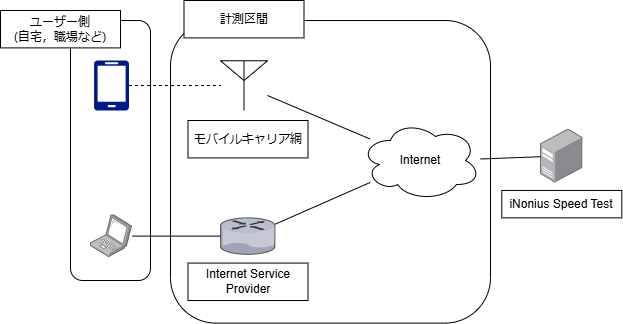
\includegraphics[width=1.0\textwidth]{fig/Measurment.png}
    \caption{iNonius Speed Testの計測区間}
    \label{fig:Measurment}
\end{figure}
\FloatBarrier
\begin{table}[htbp]
    \caption{iNonius スピードテストの計測ログの情報}
    \label{tab:loginfo}
    \begin{center}
        \begin{tabular}{c|c} \hline
            項目 & 説明 \\ \hline \hline
            userid & ユーザーを識別するID \\
            id & 計測ログを識別するID \\
            timestamp & 計測が行われた日時 \\
            ip & 計測元のIPアドレス \\
            isIpv4 & IPv4で計測されたかどうかのフラグ \\
            ispInfo & ISPに関する情報(社名,本拠地など) \\
            ua & 計測端末のOSやブラウザの情報 \\
            connectionType & Network Information APIの結果 \\
            lang & ブラウザの言語設定 \\
            dl & ダウロードのスループットの計測結果[Mbps] \\
            ul & アップロードのスループットの計測結果[Mbps] \\
            ping & RTTの計測結果[ms] \\
            jitter & RTTの揺らぎの計測結果[ms] \\
            mss & MSSのサイズ \\
            ttl & TTLの値 \\
            lossRate & パケットロス率の計測結果[\%] \\
            defaultIp & デフォルトのIP \\
            srcPort & 計測元のソースポート \\ \hline
        \end{tabular}
    \end{center}
\end{table}
\FloatBarrier
%\end{comment}

\section{アクセス環境の判定}
\label{label:accesstype}
アクセス環境は\cref{tab:accesstype} のように分類する.ISPの網の判定には,計測ログのispInfoを使用する.この値はLiberSpeedが,計測の過程でipifo.io\cite{ipinfo}に計測元のIPアドレスの情報を問い合わせて取得した情報である.IPv4/IPv6のそれぞれの計測結果に含まれるこの値を比較して判定した.

アクセス網の種類の計測ログに含まれる情報だけでは判断できないため,GeoLocation Technology が提供する「どこどこ JP」\cite{docodoco}を使用した.このサービスは.IPアドレスに地理情報や企業情報などを紐づけたデータベースで,今回使用したアクセス網の種類の判定なども含まれる.計測ログのIPアドレスを基に,このサービスを用いてアクセス網の種類を判定した.


インターネット接続方式の判定には,先行研究で用いられているMSSの値を用いた判定方法を使用した.判定の基準は\cref{tab:mss}の通りである.この表をもとに,IPv4/IPv6のそれぞれの計測結果に含まれるMSSの値でIPoEかPPPoEかを判定し,最後に組み合わせてインターネット接続方式を判定した.

%\begin{comment}
\begin{table}[htbp]
    \caption{アクセス環境の分類}
    \label{tab:accesstype}
    \begin{center}
        \begin{tabular}{c|c} \hline
            アクセス環境の分類 & 詳細な分類 \\ \hline \hline
            \multirow{2}{*}{ISPの網} & IPv4/IPv6で同じ場合 \\
            & IPv4/IPv6で異なる場合 \\
            \hline
            \multirow{3}{*}{アクセス網の種類} & FTTH \\ 
            & CATV \\
            & Mobile \\
            \hline
            \multirow{3}{*}{インターネット接続方式} & IPv4/IPv6共にIPoE \\
            & IPv4/IPv6共にPPPoE \\
            & IPv4がPPPoE,IPv6がIPoE \\ \hline
        \end{tabular}
    \end{center}
\end{table}
\FloatBarrier
\begin{table}[htbp]
    \caption{インターネット接続方式の判定とMSSの値}
    \label{tab:mss}
    \begin{center}
        \begin{tabular}{cc|cc} \hline
            \multicolumn{2}{c|}{インターネット接続方式}& \multicolumn{2}{c}{MSSのサイズ} \\ \hline
            IPv4& IPv6& IPv4& IPv6 \\ \hline \hline
            IPoE & IPoE & 1460 & 1440 \\
            PPPoE & PPPoE & 1452 & 1394 \\
            PPPoE & IPoE & 1452 & 1440 \\ \hline
        \end{tabular}
    \end{center}
\end{table}
\FloatBarrier
%\end{comment}

\section{スループットの調査}
\label{sec:throughput}
\cref{label:accesstype}で示したアクセス環境の違いによる集計結果を IPv4 と IPv6 のスループットの比較がわかるように\cref{fig:old_isp_dl}のように散布図とヒストグラムのグラフにして分析した.左下が IPv4 と IPv6 のスループットの相関を示す散布図で,左上と右下のヒストグラムがそれぞれ IPv4 と IPv6 のスループットの階級ごとの度数を表す.散布図の縦軸と右下のヒストグラムの縦軸,散布図の横軸と左上のヒストグラムの横軸はそれぞれ同じスケールになっている.
また,各グラフの右上に,データ数$N$, 相関係数$r$,IPv6/IPv4の平均スループットおよび最大スループットの数値を示す.

%%%%%%%%%%%%%%%%%%%%%%%%%%%%%%%%%%%%%%%%%%%%%%%%%%%%%%%%%%%%%%%%%%%%%%%%%%
\subsection{ISPの網によるスループットへの影響}
\label{subsec:isp_dl}
\cref{fig:old_isp_dl,fig:new_isp_dl} はそれぞれの期間のISPの網の違いによるダウンロードのスループットの比較を示す.ただし,ここで言う「ISPの網の違い」とはIPv4とIPv6で同じISPを使用した場合と異なるISPを使用した場合の2つを指す.\cref{fig:old_isp_dl} は{\bf 期間(1)},\cref{fig:new_isp_dl} は{\bf 期間(2)}の結果である.\cref{old_sameISP_dl,new_sameISP_dl}は同じISPを使用した場合の結果で,\cref{old_diffISP_dl,new_diffISP_dl}は異なるISPを使用した場合の結果である.

\cref{old_sameISP_dl,old_diffISP_dl}を比較するとIPv4/IPv6のスループットの相関性に違いが見られる.これは\cref{fig:new_isp_dl}でも同様である.\cref{fig:old_isp_ul,fig:new_isp_ul}のそれぞれの(a)と(b)を比較すると,ダウンロードに比べて相関係数の値の差が小さいが概ね同様の傾向が見られる.
(b)の場合は,IPv4/IPv6で異なるISPであることから計測サーバーへの経路が異なる可能性があり,その結果IPv4/IPv6で相関性が低くなると考えられる.
そこで,ISPによってふるまいが異なる可能性があるのか確認するためにデータ数の多い3社に絞って分析を行う.ただし,データ数の都合上(2)の期間のみである.\cref{fig:new_isp_dl2,fig:new_isp_ul2}はそれぞれA社,B社,C社のISPの違いによるダウンロードとアップロードのスループットの比較を示す.3社ともそれぞれのIPv4/IPv6の間の相関性は高く,それぞれのヒストグラムの形も似ている.しかし異なるISP同士で比較すると,ヒストグラムのピークの現れる位置が異なることから,ISPによってふるまいが異なる可能性があることがわかる.

%\begin{comment}
\begin{figure}[htbp]
    \begin{center}
        \begin{subfigure}[b]{0.49\textwidth}
            \centering
            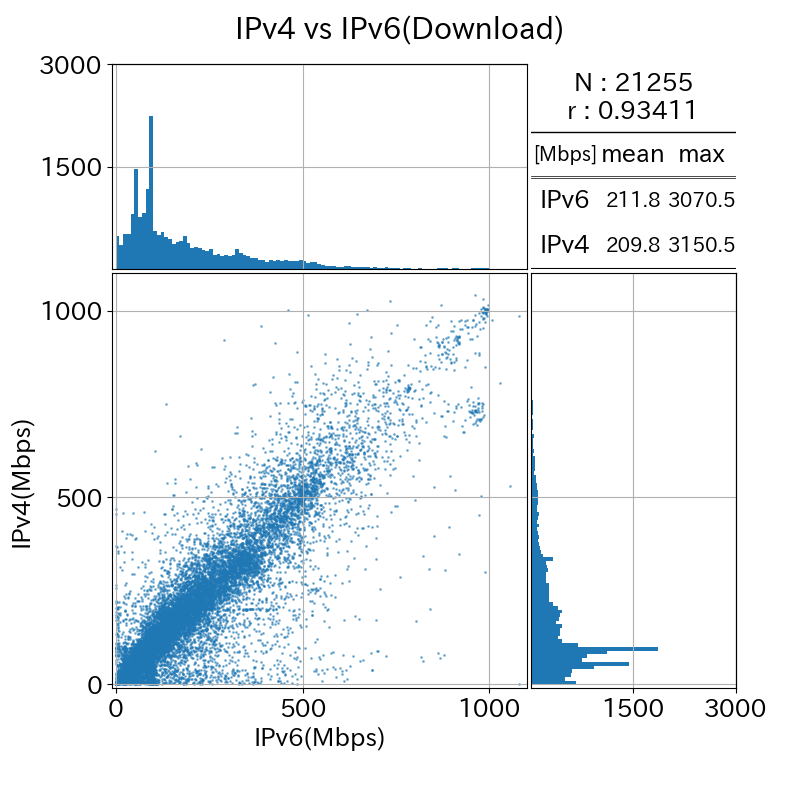
\includegraphics[width=1.0\textwidth]{fig/old_sameISP_dl.png}
            \subcaption{同じISPを使用した場合}
            \label{old_sameISP_dl}
        \end{subfigure}
        \begin{subfigure}[b]{0.49\textwidth}
            \centering
            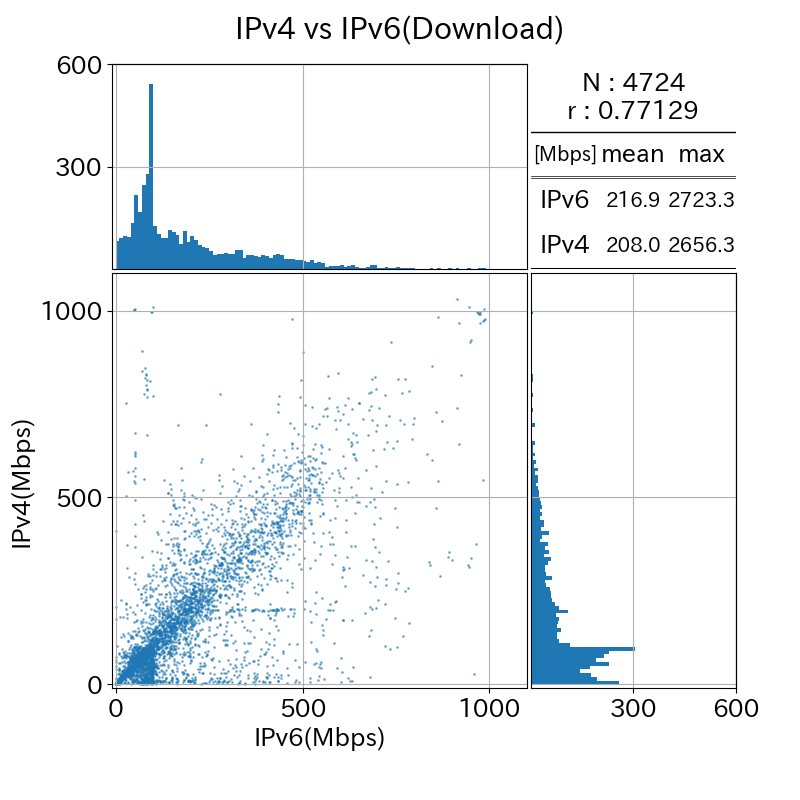
\includegraphics[width=1.0\textwidth]{fig/old_diffISP_dl.png}
            \subcaption{異なるISPを使用した場合}
            \label{old_diffISP_dl}
        \end{subfigure}
        \caption{{\bf 期間(1)}におけるダウンロードのスループット}
        \label{fig:old_isp_dl}
    
        \begin{subfigure}[b]{0.49\textwidth}
            \centering
            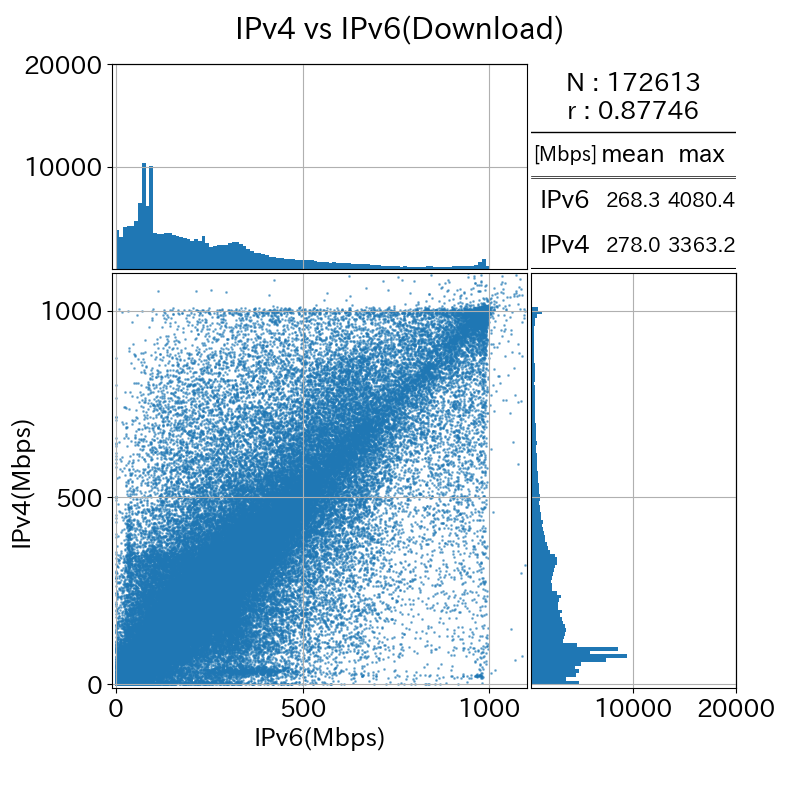
\includegraphics[width=1.0\textwidth]{fig/new_sameISP_dl.png}
            \subcaption{同じISPを使用した場合}
            \label{new_sameISP_dl}
        \end{subfigure}
        \begin{subfigure}[b]{0.49\textwidth}
            \centering
            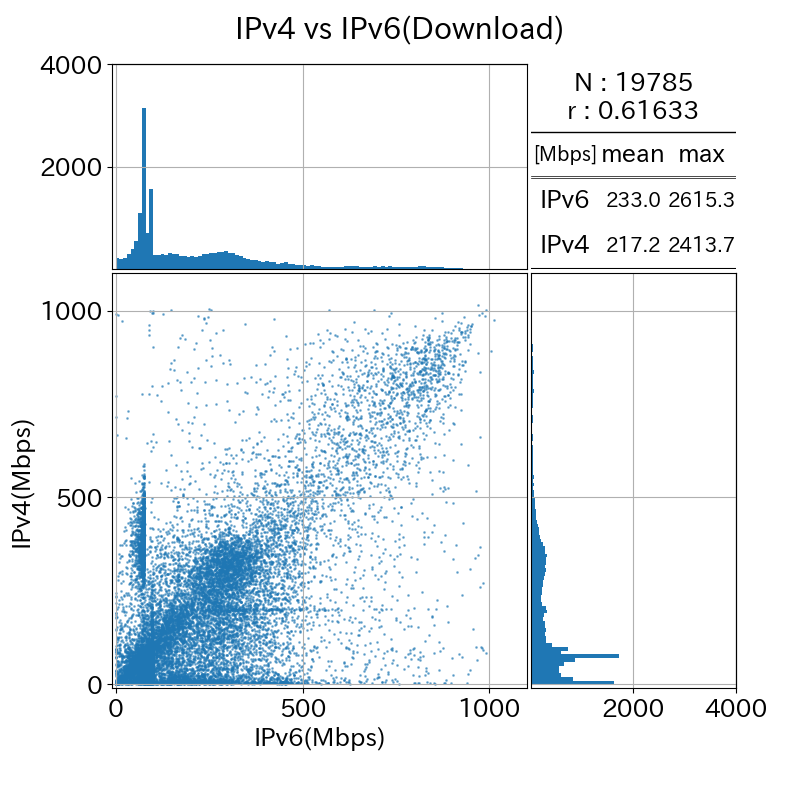
\includegraphics[width=1.0\textwidth]{fig/new_diffISP_dl.png}
            \subcaption{異なるISPを使用した場合}
            \label{new_diffISP_dl}
        \end{subfigure}
        \caption{{\bf 期間(2)}におけるダウンロードのスループット}
        \label{fig:new_isp_dl}
    \end{center}
\end{figure}
\FloatBarrier

\begin{figure}[htbp]
    \begin{center}
        \begin{subfigure}[b]{0.49\textwidth}
            \centering
            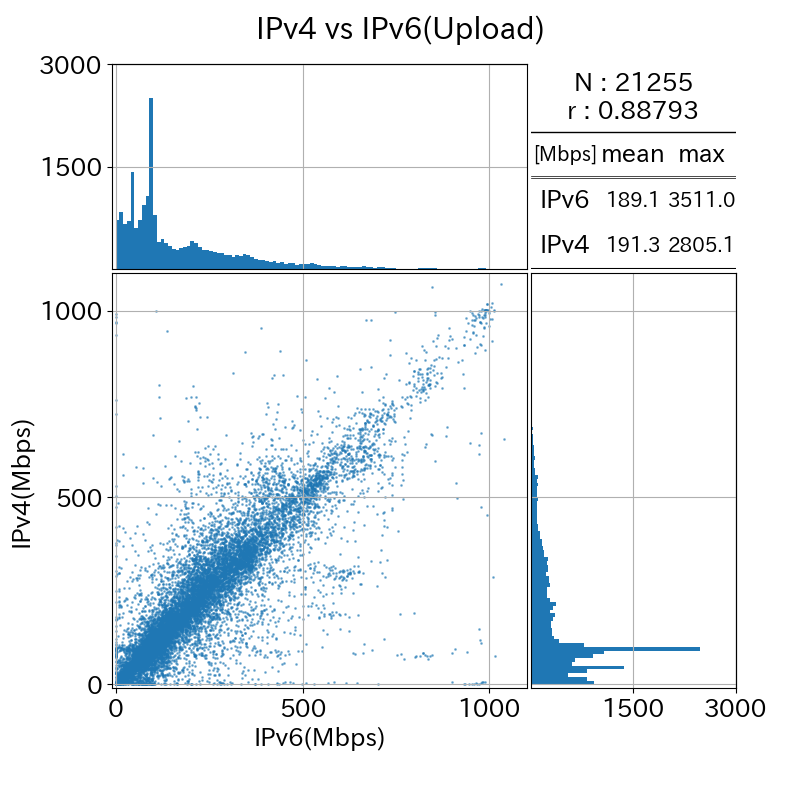
\includegraphics[width=1.0\textwidth]{fig/old_sameISP_ul.png}
            \subcaption{同じISPを使用した場合}
            \label{old_sameISP_ul}
        \end{subfigure}
        \begin{subfigure}[b]{0.49\textwidth}
            \centering
            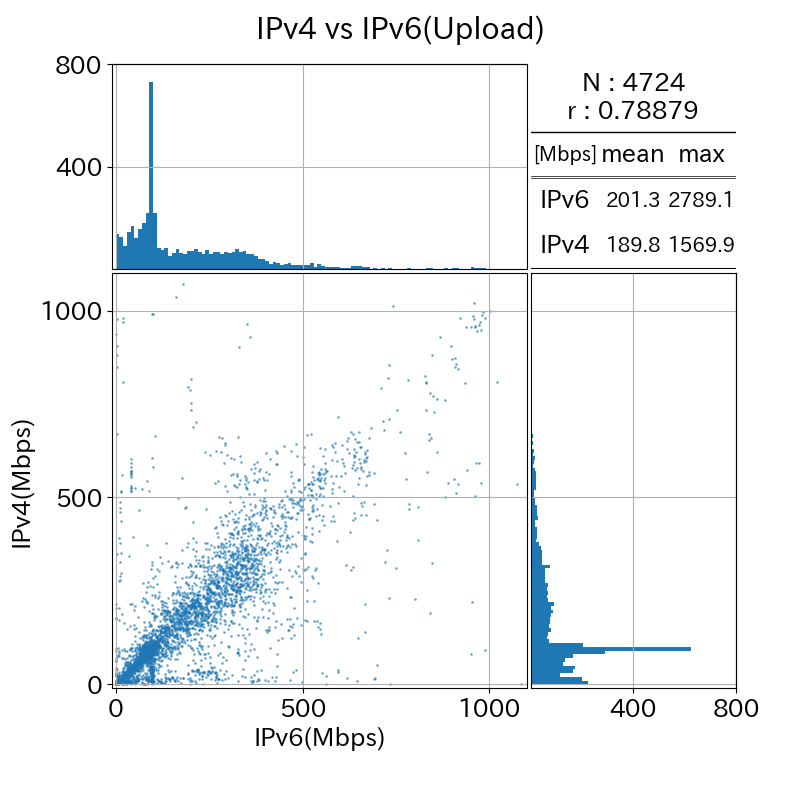
\includegraphics[width=1.0\textwidth]{fig/old_diffISP_ul.png}
            \subcaption{異なるISPを使用した場合}
            \label{old_diffISP_ul}
        \end{subfigure}
        \caption{{\bf 期間(1)}におけるアップロードのスループット}
        \label{fig:old_isp_ul}

        \begin{subfigure}[b]{0.49\textwidth}
            \centering
            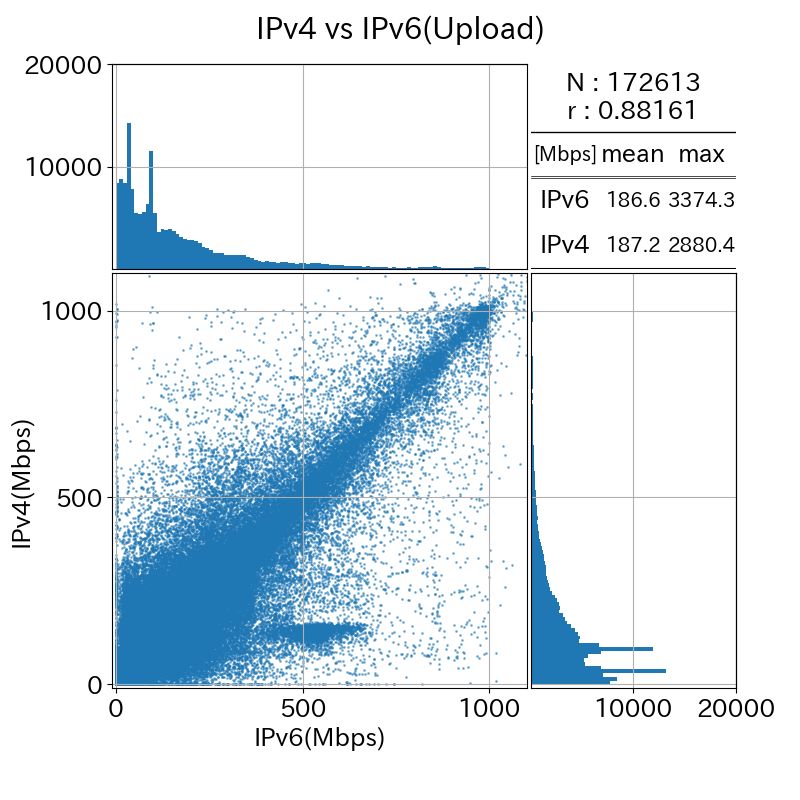
\includegraphics[width=1.0\textwidth]{fig/new_sameISP_ul.png}
            \subcaption{同じISPを使用した場合}
            \label{new_sameISP_ul}
        \end{subfigure}
        \begin{subfigure}[b]{0.49\textwidth}
            \centering
            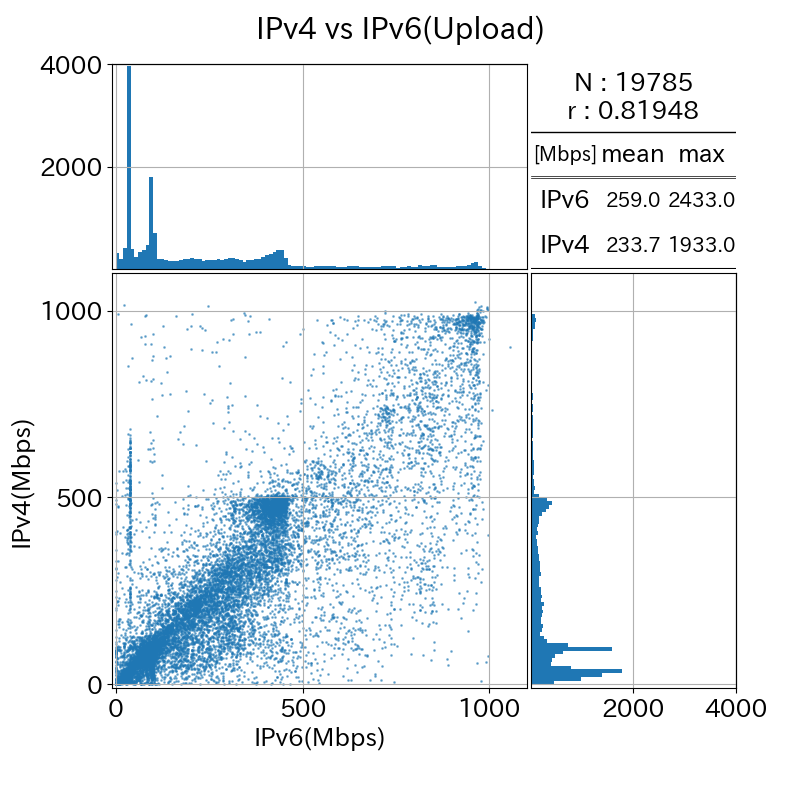
\includegraphics[width=1.0\textwidth]{fig/new_diffISP_ul.png}
            \subcaption{異なるISPを使用した場合}
            \label{new_diffISP_ul}
        \end{subfigure}
        \caption{{\bf 期間(2)}におけるアップロードのスループット}
        \label{fig:new_isp_ul}
    \end{center}
\end{figure}
\FloatBarrier

\begin{figure}[htbp]
    %\centering
    \begin{center}
        % 左側の図
        \begin{minipage}[t]{0.48\textwidth}
            \begin{center}
                \begin{subfigure}[b]{\textwidth}
                    \centering
                    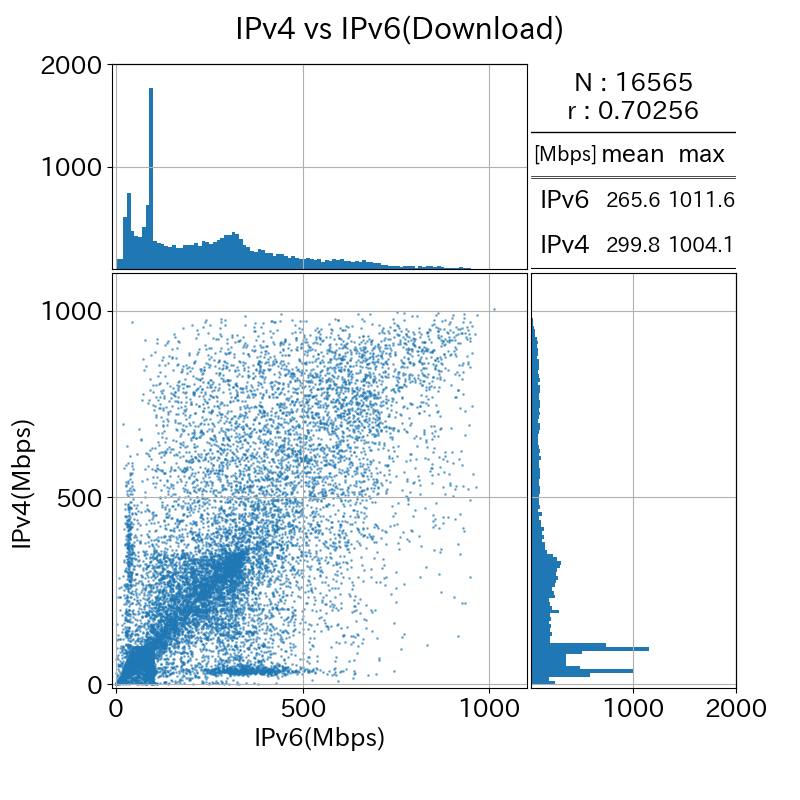
\includegraphics[width=0.85\textwidth]{fig/new_NTT_dl.png}
                    \subcaption{A社の場合}
                    \label{new_NTT_dl}
                    \end{subfigure}
                \begin{subfigure}[b]{\textwidth}
                    \centering
                    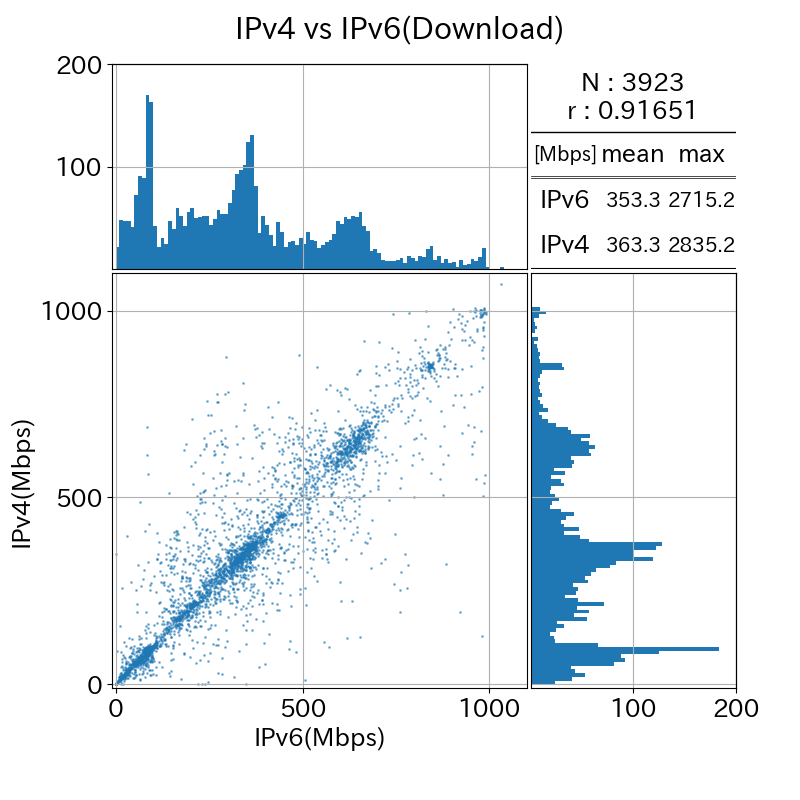
\includegraphics[width=0.85\textwidth]{fig/new_KDDI_dl.png}
                    \subcaption{B社の場合}
                    \label{new_KDDI_dl}
                \end{subfigure}
                \begin{subfigure}[b]{\textwidth}
                    \centering
                    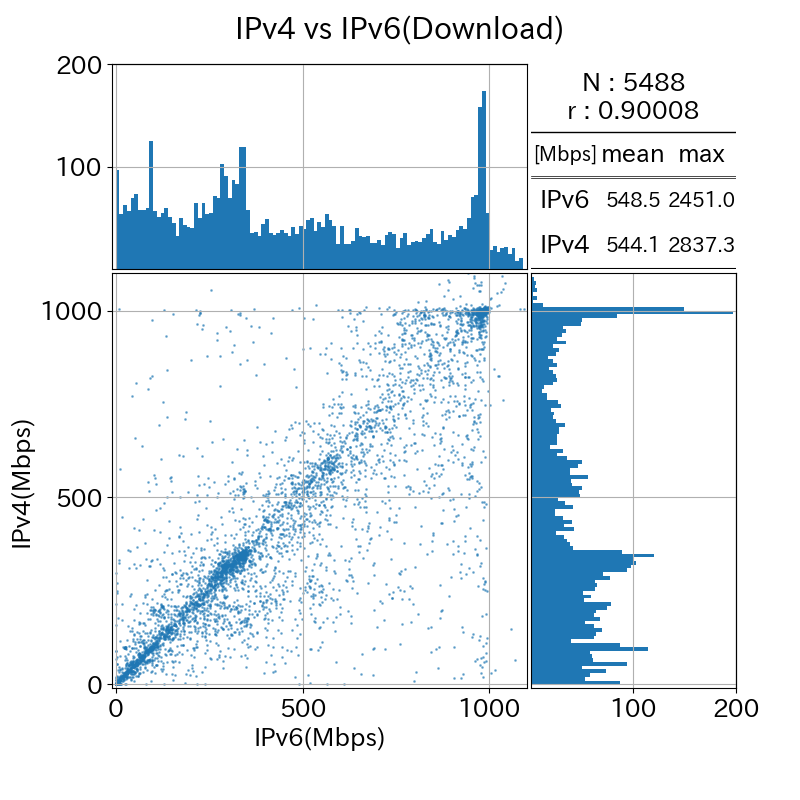
\includegraphics[width=0.85\textwidth]{fig/new_Sony_dl.png}
                    \subcaption{C社の場合}
                    \label{new_Sony_dl}
                \end{subfigure}
                \caption{ISPの違いによる\\ダウンロードのスループット}
                \label{fig:new_isp_dl2}
            \end{center}
        \end{minipage}
        \hfill
        % 右側の図
        \begin{minipage}[t]{0.48\textwidth}
            \begin{center}
                \begin{subfigure}[b]{\textwidth}
                    \centering
                    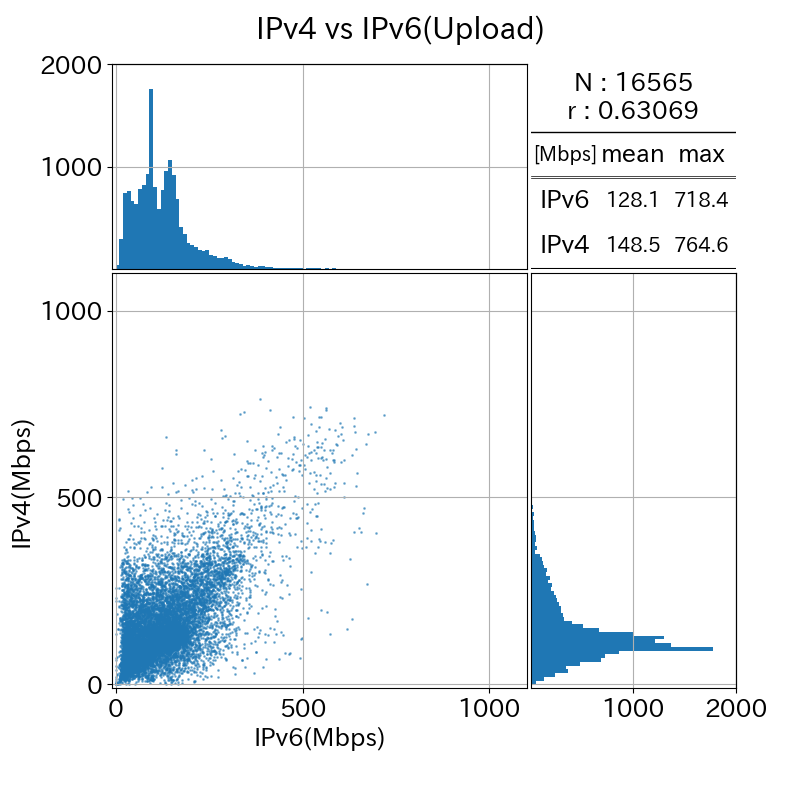
\includegraphics[width=0.85\textwidth]{fig/new_NTT_ul.png}
                    \subcaption{A社の場合}
                    \label{new_NTT_ul}
                \end{subfigure}
                \begin{subfigure}[b]{\textwidth}
                    \centering
                    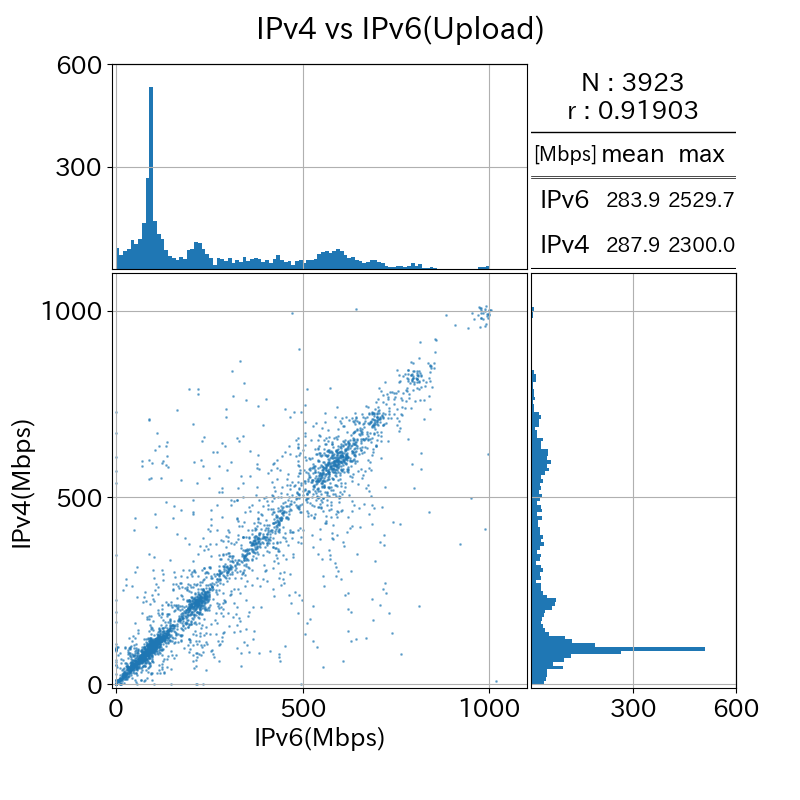
\includegraphics[width=0.85\textwidth]{fig/new_KDDI_ul.png}
                    \subcaption{B社の場合}
                    \label{new_KDDI_ul}
                \end{subfigure}
                \begin{subfigure}[b]{\textwidth}
                    \centering
                    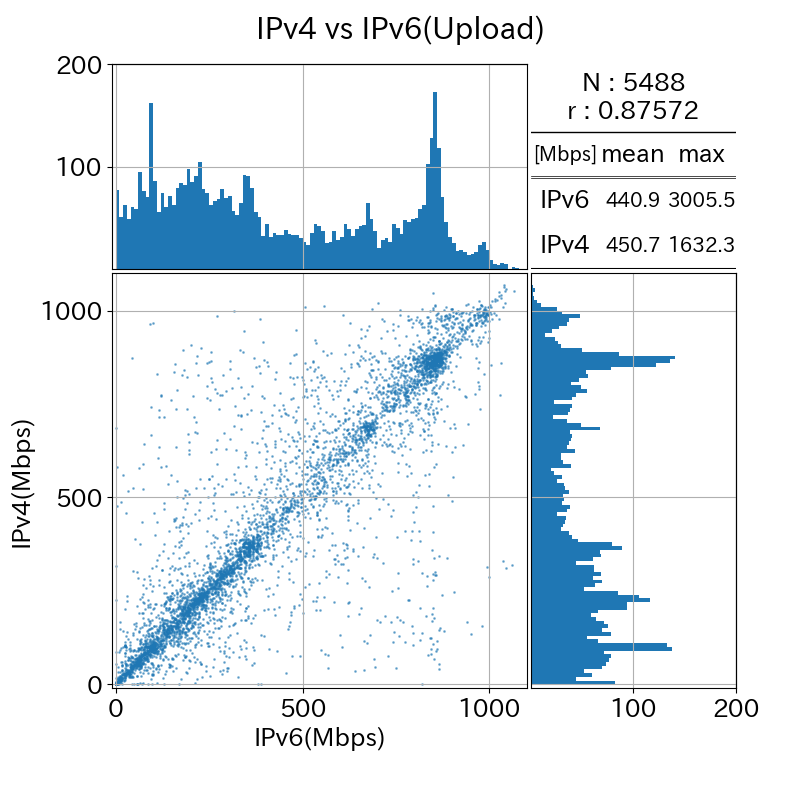
\includegraphics[width=0.85\textwidth]{fig/new_Sony_ul.png}
                    \subcaption{C社の場合}
                    \label{new_Sony_ul}
                \end{subfigure}
                \caption{ISPの違いによる\\アップロードのスループット}
                \label{fig:new_isp_ul2}
            \end{center}
        \end{minipage}
    \end{center}
\end{figure}
\FloatBarrier
%\end{comment}

%%%%%%%%%%%%%%%%%%%%%%%%%%%%%%%%%%%%%%%%%%%%%%%%%%%%%%%%%%%%%%%%%%%%%%%%%%
\subsection{アクセス網の種類によるスループットへの影響}
次にアクセス網の種類によるスループットへの影響について述べる.\cref{fig:old_Line_dl,fig:new_Line_dl}はダウンロードのスループットのグラフ,\cref{fig:old_Line_ul,fig:new_Line_ul}はアップロードのスループットのグラフである.\cref{old_FTTH_dl,new_FTTH_dl}はそれぞれの期間でFTTHを使用した場合のダウンロードのスループットである.両者とも100Mbps付近にピークが表れて緩やかにデータ数が減っていくふるまいを見せている.これはアップロードの場合も類似する振る舞いをしている.一方,\cref{old_CATV_dl,new_CATV_dl}のCATVを使用した場合はピークが表れる位置がFTTHと異なり,ダウンロードの場合は340Mbps付近に表れる.アップロードの場合は10Mbpsにピークが表れている.CATVを使用したインターネット接続サービスについて調査すると,ダウンロードのスループットが最大340Mbps,アップロードのスループットが最大10Mbpsであると述べているサービスがいくつか確認された.このことからアクセス網の種類によってスループットの限界が異なることがわかる.さらに\cref{new_Mobile_dl,new_Mobile_ul}のMobileの場合は10Mbps付近にピークが表れている.Mobileを使用した場合のスループットの限界はFTTHやCATVに比べて低いことがわかる.ただし,\cref{old_CATV_dl,new_CATV_dl}を比較すると,340Mbpsのピークの前後のヒストグラムの振る舞いが異なる.ピークの前後のデータの割合は\cref{tab:catv}のように変化し340Mbps以上のデータが約20\%増加している.CATVによる配信サービスについて調べると,旧来使用されてきたHFC(Hybrid Fiber-Coaxial)方式や同軸方式を光ファイバーに置き換える動き\cite{nagaoka}が進んでおり,総務省の資料\cite{catv}によると約80\%の事業者がFTTH方式を採用していることがわかった.このことから,アクセス網の種類だけでなくアクセス環境全体が時期によって変化していることがわかる.
以上のことからアクセス網の種類によってスループットの限界が異なることがわかったが,その振る舞いは時期によって異なることがわかる.

%\begin{comment}
\begin{figure}[htbp]
    %\centering
    \begin{center}
        % 左側の図
        \begin{minipage}[t]{0.48\textwidth}
            \begin{center}
                \begin{subfigure}[b]{\textwidth}
                    \centering
                    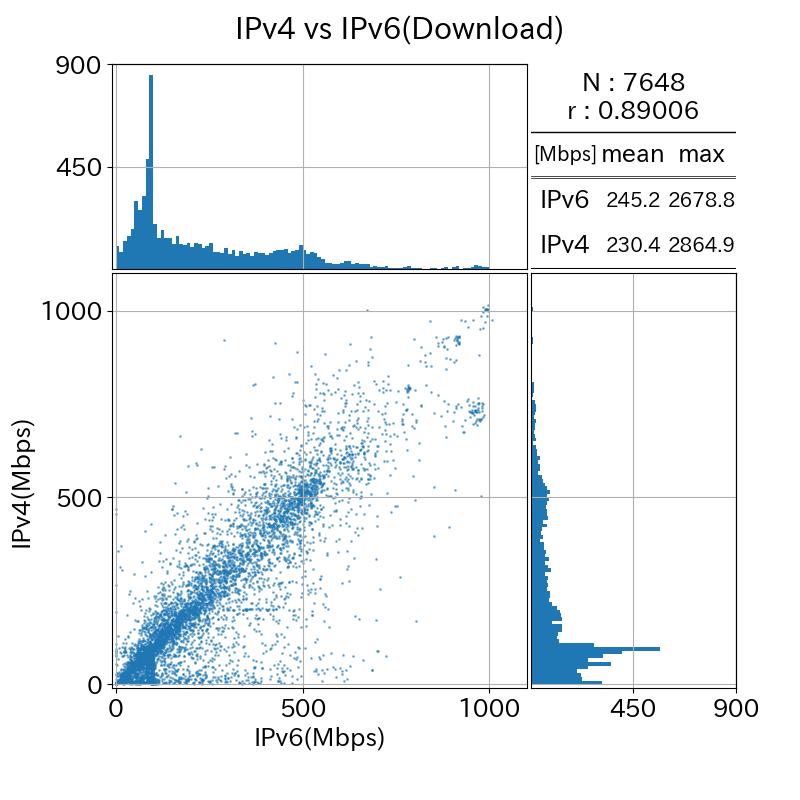
\includegraphics[width=0.85\textwidth]{fig/old_FTTH_dl.png}
                    \subcaption{FTTHを使用した場合}
                    \label{old_FTTH_dl}
                \end{subfigure}
                \begin{subfigure}[b]{\textwidth}
                    \centering
                    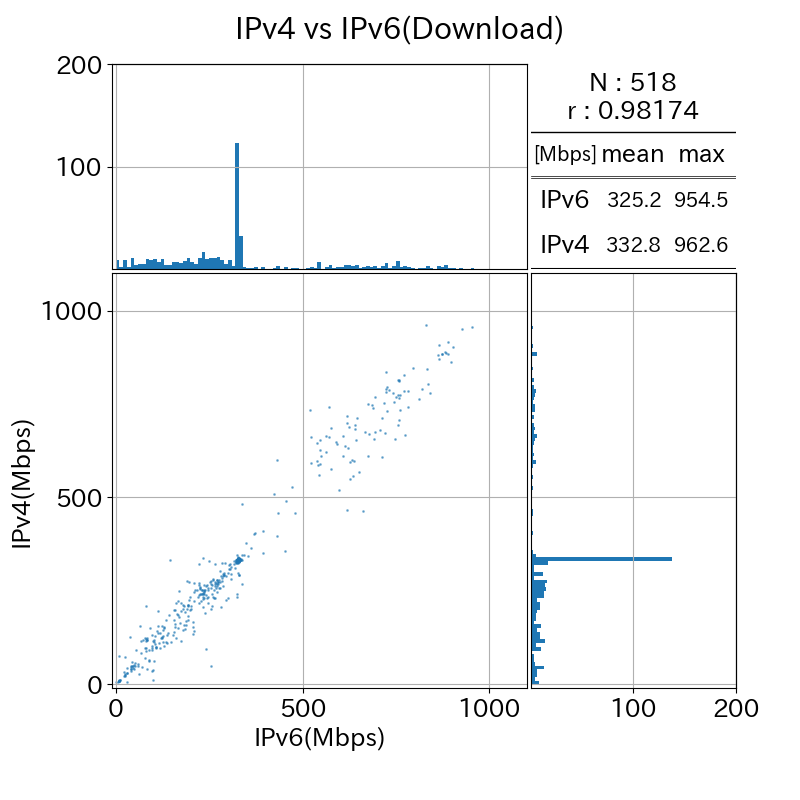
\includegraphics[width=0.85\textwidth]{fig/old_CATV_dl.png}
                    \subcaption{CATVを使用した場合}
                    \label{old_CATV_dl}
                \end{subfigure}
                \begin{subfigure}[b]{\textwidth}
                    \centering
                    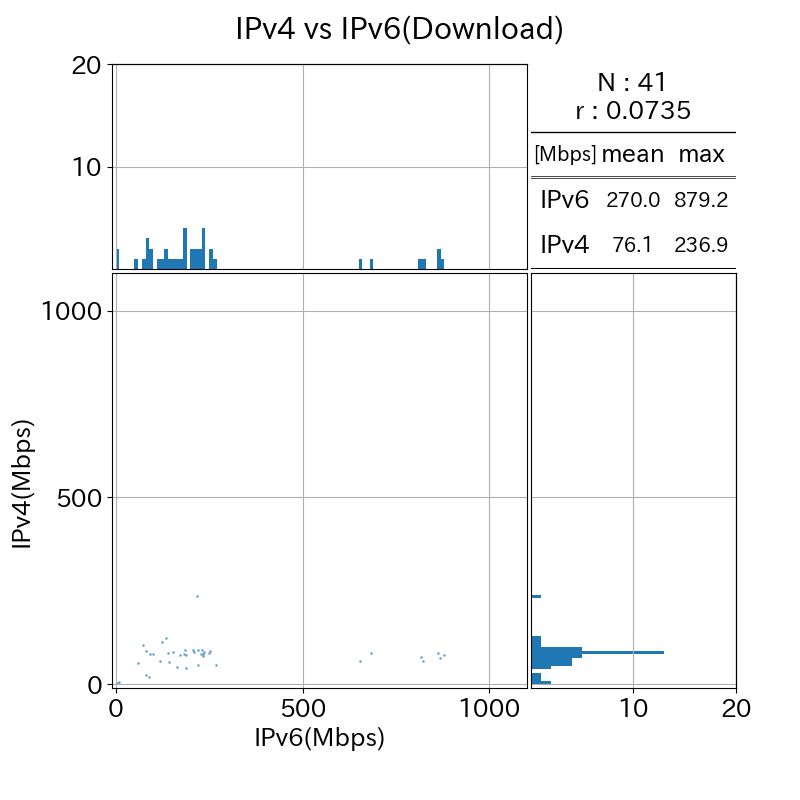
\includegraphics[width=0.85\textwidth]{fig/old_Mobile_dl.png}
                    \subcaption{Mobileを使用した場合}
                    \label{old_Mobile_dl}
                \end{subfigure}
            \caption{(1)のダウンロードのスループット}
            \label{fig:old_Line_dl}
            \end{center}
        \end{minipage}
        \hfill
        \begin{minipage}[t]{0.48\textwidth}
            \begin{subfigure}[b]{\textwidth}
                \centering
                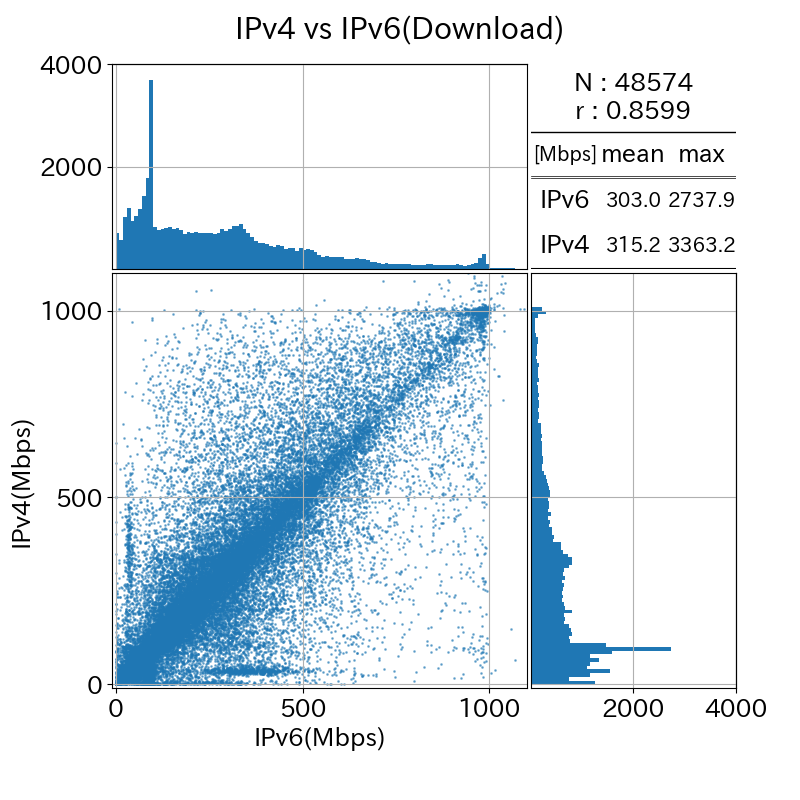
\includegraphics[width=0.85\textwidth]{fig/new_FTTH_dl.png}
                \subcaption{FTTHを使用した場合}
                \label{new_FTTH_dl}
            \end{subfigure}
            \begin{subfigure}[b]{\textwidth}
                \centering
                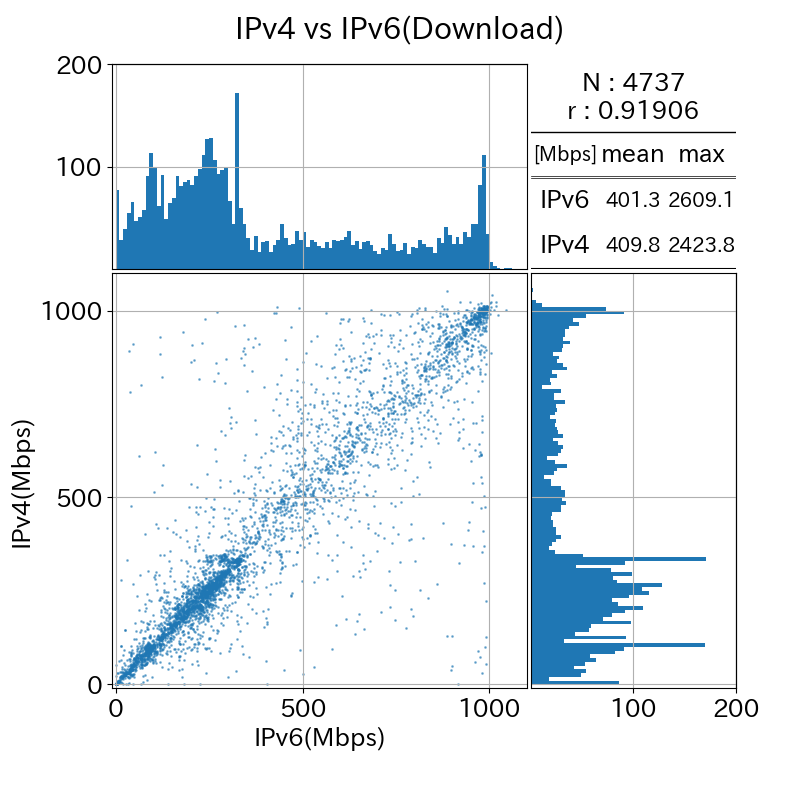
\includegraphics[width=0.85\textwidth]{fig/new_CATV_dl.png}
                \subcaption{CATVを使用した場合}
                \label{new_CATV_dl}
            \end{subfigure}
            \begin{subfigure}[b]{\textwidth}
                \centering
                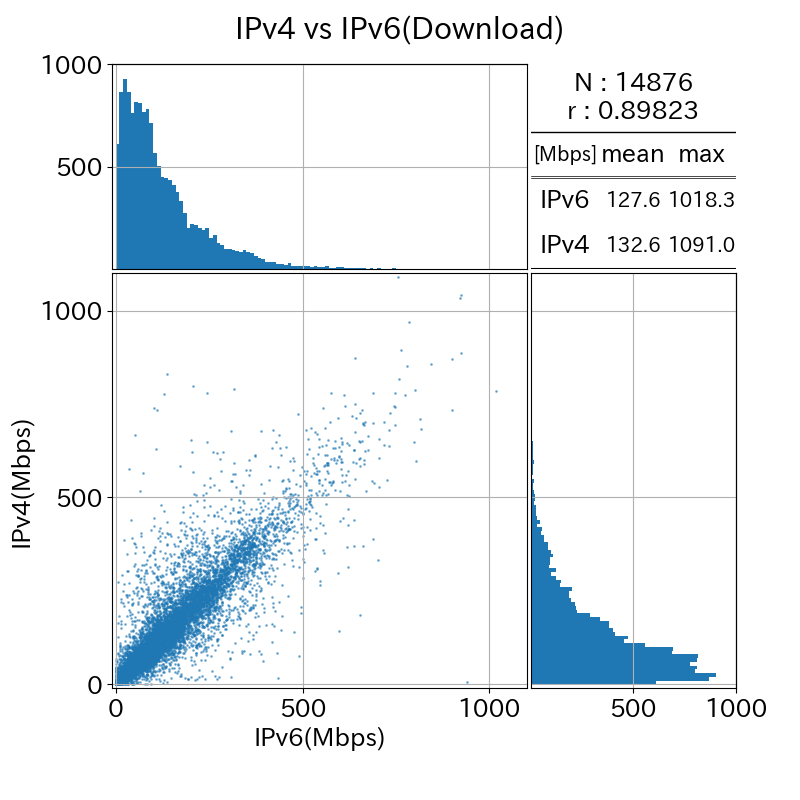
\includegraphics[width=0.85\textwidth]{fig/new_Mobile_dl.png}
                \subcaption{Mobileを使用した場合}
                \label{new_Mobile_dl}
            \end{subfigure}
            \caption{(2)のダウンロードのスループット}
            \label{fig:new_Line_dl}
        \end{minipage}
    \end{center}
\end{figure}
\FloatBarrier

\begin{figure}[htbp]
    %\centering
    \begin{center}
        % 左側の図
        \begin{minipage}[t]{0.48\textwidth}
            \begin{center}
                \begin{subfigure}[b]{\textwidth}
                    \centering
                    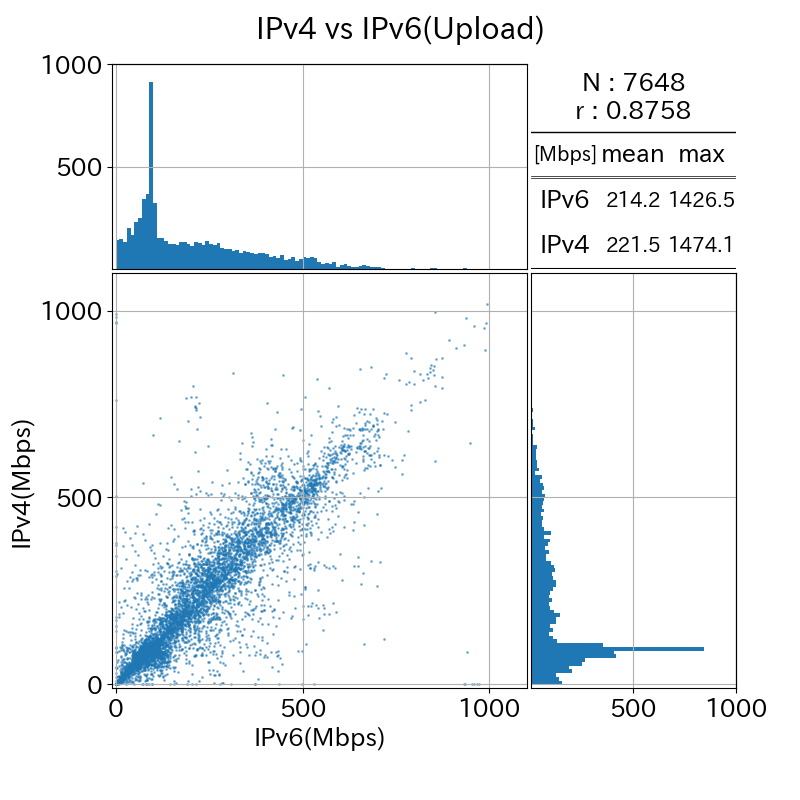
\includegraphics[width=0.85\textwidth]{fig/old_FTTH_ul.png}
                    \subcaption{FTTHを使用した場合}
                    \label{old_FTTH_ul}
                \end{subfigure}
                \begin{subfigure}[b]{\textwidth}
                    \centering
                    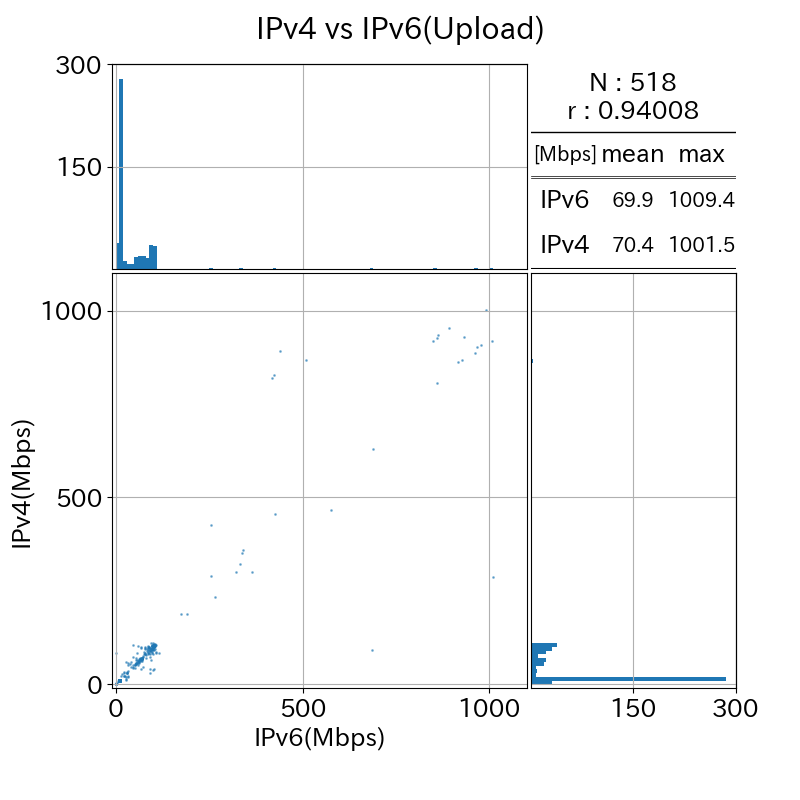
\includegraphics[width=0.85\textwidth]{fig/old_CATV_ul.png}
                    \subcaption{CATVを使用した場合}
                    \label{old_CATV_ul}
                \end{subfigure}
                \begin{subfigure}[b]{\textwidth}
                    \centering
                    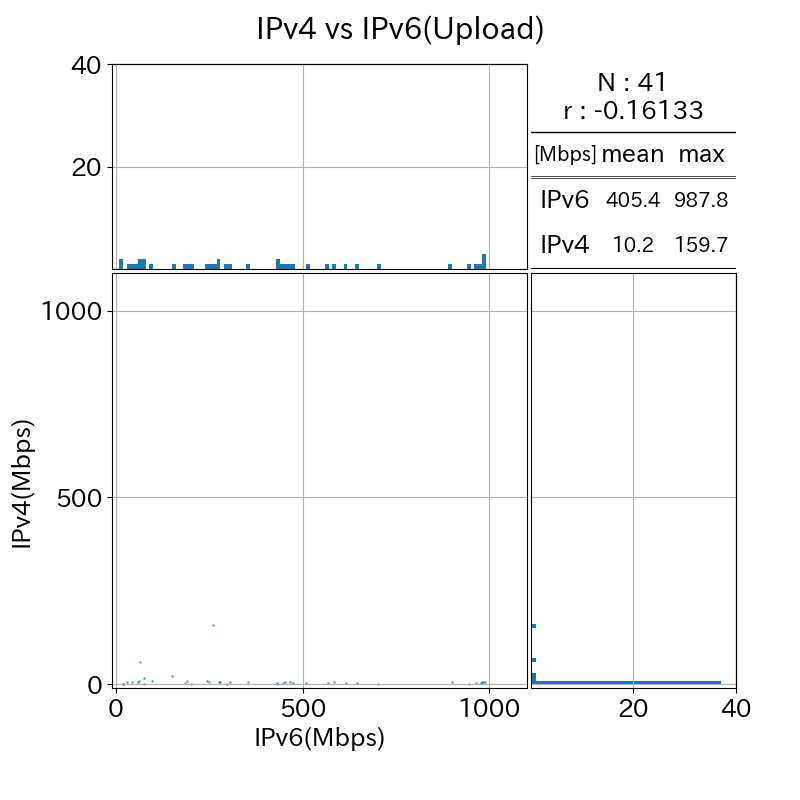
\includegraphics[width=0.85\textwidth]{fig/old_Mobile_ul.png}
                    \subcaption{Mobileを使用した場合}
                    \label{old_Mobile_ul}
                \end{subfigure}
            \caption{(1)のアップロードのスループット}
            \label{fig:old_Line_ul}
            \end{center}
        \end{minipage}
        \hfill
        \begin{minipage}[t]{0.48\textwidth}
            \begin{subfigure}[b]{\textwidth}
                \centering
                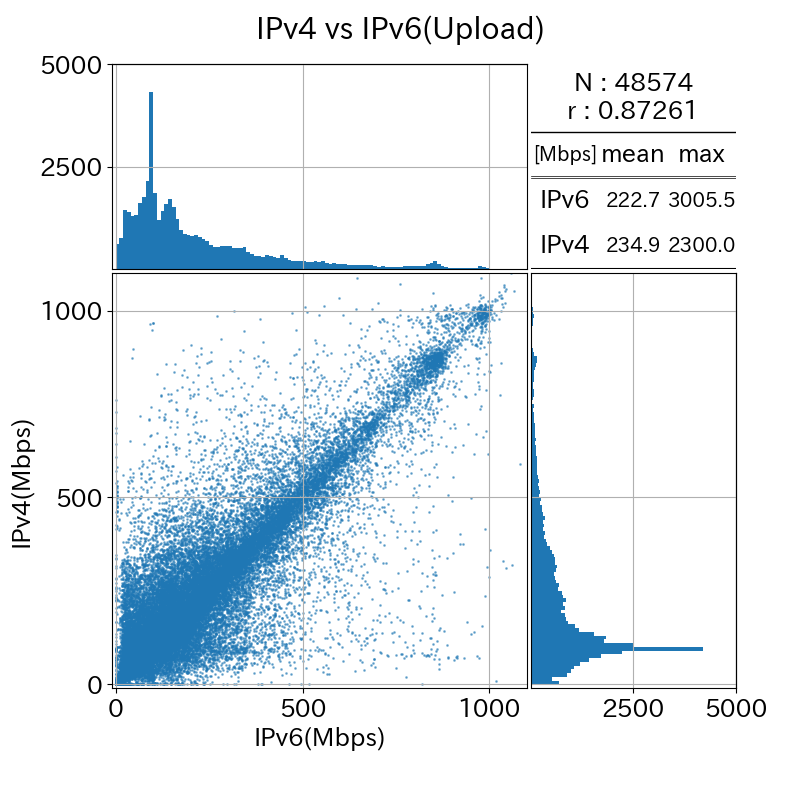
\includegraphics[width=0.85\textwidth]{fig/new_FTTH_ul.png}
                \subcaption{FTTHを使用した場合}
                \label{new_FTTH_ul}
            \end{subfigure}
            \begin{subfigure}[b]{\textwidth}
                \centering
                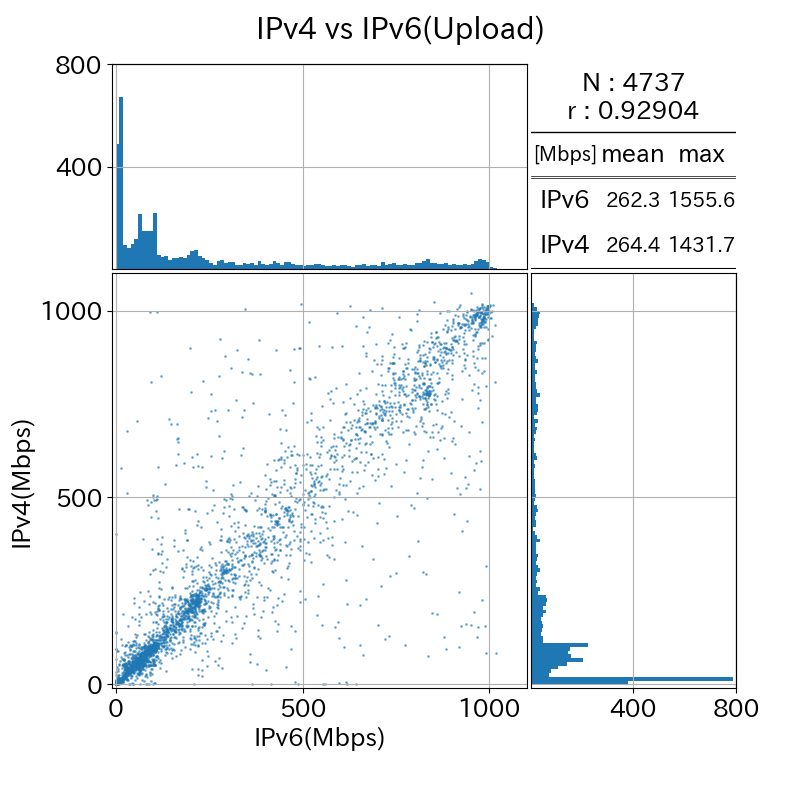
\includegraphics[width=0.85\textwidth]{fig/new_CATV_ul.png}
                \subcaption{CATVを使用した場合}
                \label{new_CATV_ul}
            \end{subfigure}
            \begin{subfigure}[b]{\textwidth}
                \centering
                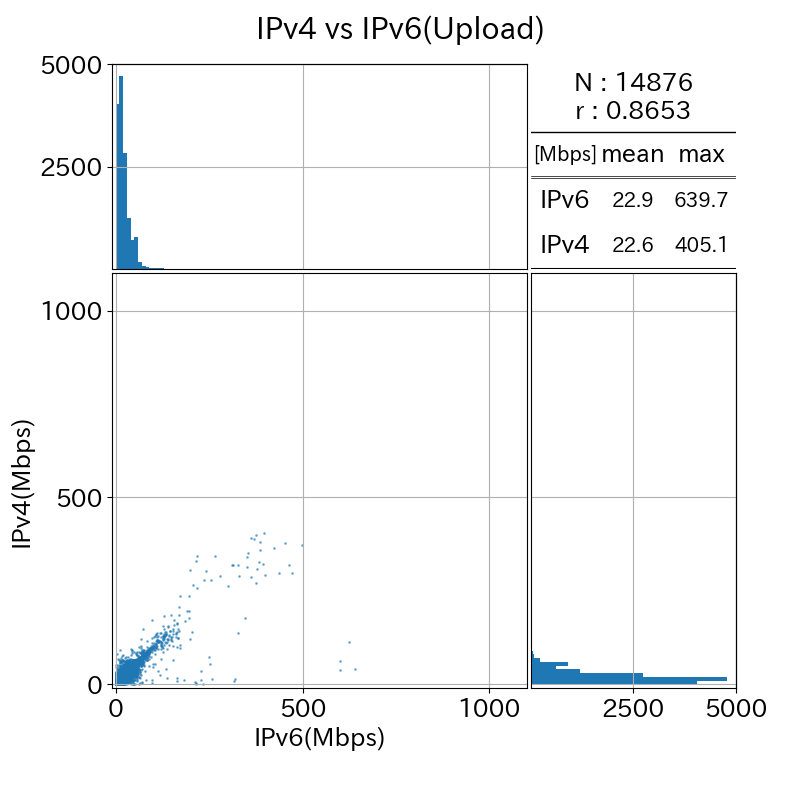
\includegraphics[width=0.85\textwidth]{fig/new_Mobile_ul.png}
                \subcaption{Mobileを使用した場合}
                \label{new_Mobile_ul}
            \end{subfigure}
            \caption{(2)のアップロードのスループット}
            \label{fig:new_Line_ul}
        \end{minipage}
    \end{center}
\end{figure}
\FloatBarrier

\begin{table}[htbp]
    \caption{CATVのピーク前後のデータの割合}
    \label{tab:catv}
    \begin{center}
        \begin{tabular}{ccc} \hline
            期間 & 340Mbps未満のデータの割合 & 340Mbps以上のデータの割合 \\ \hline \hline
            (1) & 77.11\% & 22.89\% \\
            (2) & 57.84\% & 42.16\% \\ \hline
        \end{tabular}
    \end{center}
\end{table}
\FloatBarrier
%\end{comment}

%%%%%%%%%%%%%%%%%%%%%%%%%%%%%%%%%%%%%%%%%%%%%%%%%%%%%%%%%%%%%%%%%%%%%%%%%%
\subsection{インターネット接続方式によるスループットへの影響}
最後にインターネット接続方式によるスループットへの影響について述べる.\cref{fig:old_connect_dl,fig:new_connect_dl}はそれぞれの期間のダウンロードのスループットのグラフ,\cref{fig:old_connect_ul,fig:new_connect_ul}はアップロードのスループットのグラフである.\subref{old_IPv4aaS_dl}から\subref{old_PPPoE_dl}の平均値を比較するとIPv4とIPv6の両者とも異なる値を示している.ここで\subref{old_IPv4aaS_dl}と\subref{old_mix_dl}の条件の違いはIPv4の接続方式であるにも関わらず,IPv6のスループットの平均値も異なる.同様に\subref{old_mix_dl}と\subref{old_PPPoE_dl}の条件の違いはIPv6の接続方式であるにも関わらず,IPv4のスループットの平均値も異なる.このことからインターネットの接続方式による振る舞いの違いが表れるだけでなく,IPv4/IPv6の接続方式の組み合わせによっても振る舞いが異なることがわかる.しかし,この影響の要因は他にも検証が必要であると考える.

%\begin{comment}
\begin{figure}[htbp]
    %\centering
    \begin{center}
        % 左側の図
        \begin{minipage}[t]{0.48\textwidth}
            \begin{subfigure}[b]{\textwidth}
                \centering
                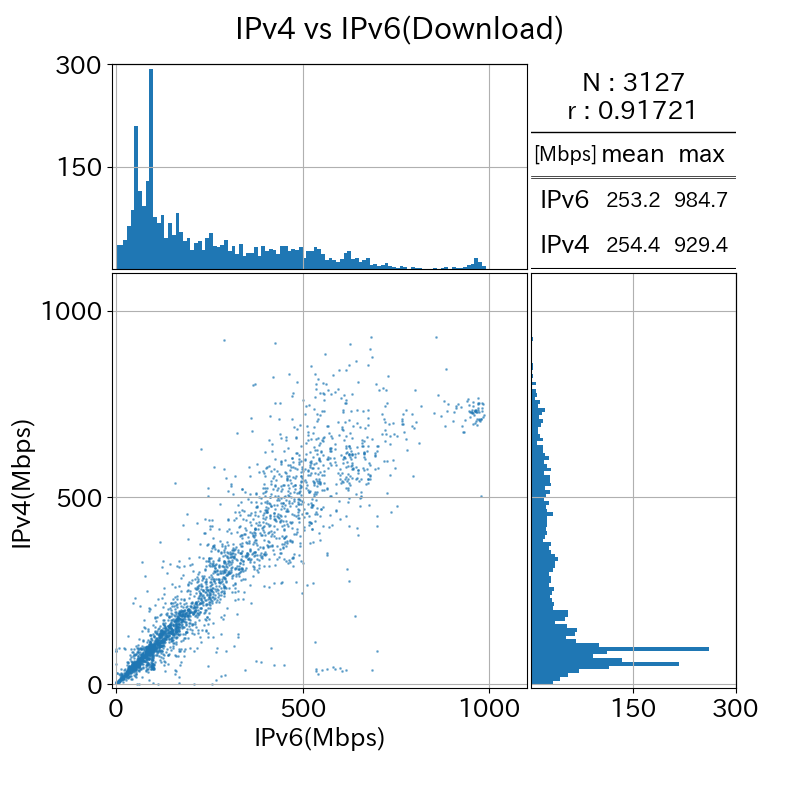
\includegraphics[width=0.8\textwidth]{fig/old_IPv4aaS_dl.png}
                \subcaption{IPv4/IPv6でIPoEを使用した場合}
                \label{old_IPv4aaS_dl}
            \end{subfigure}
            \begin{subfigure}[b]{\textwidth}
                \centering
                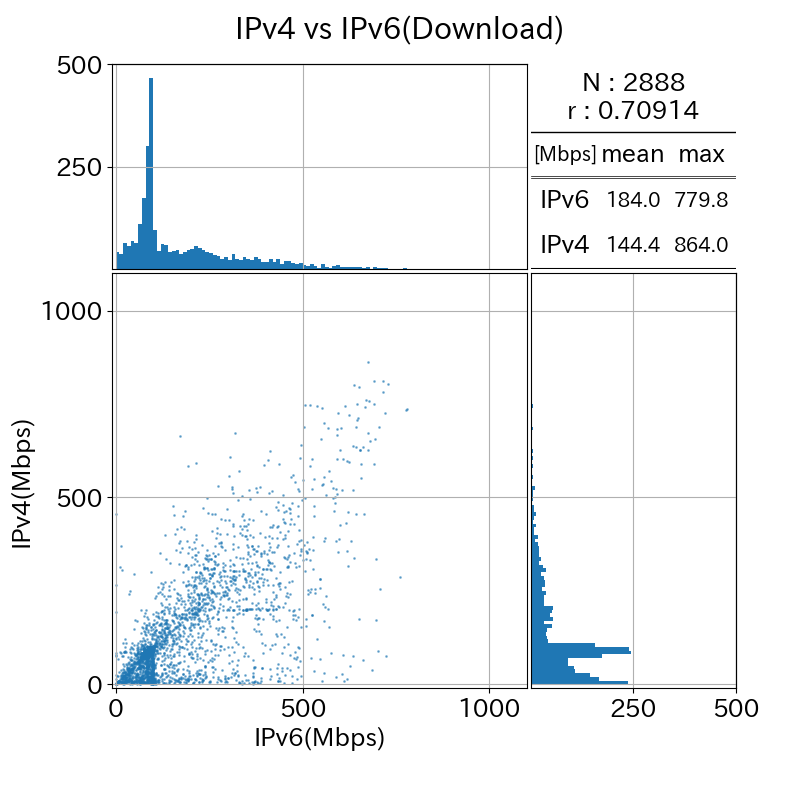
\includegraphics[width=0.8\textwidth]{fig/old_mix_dl.png}
                \subcaption{IPv4はPPPoE,IPv6はIPoEを\\使用した場合}
                \label{old_mix_dl}
            \end{subfigure}
            \begin{subfigure}[b]{\textwidth}
                \centering
                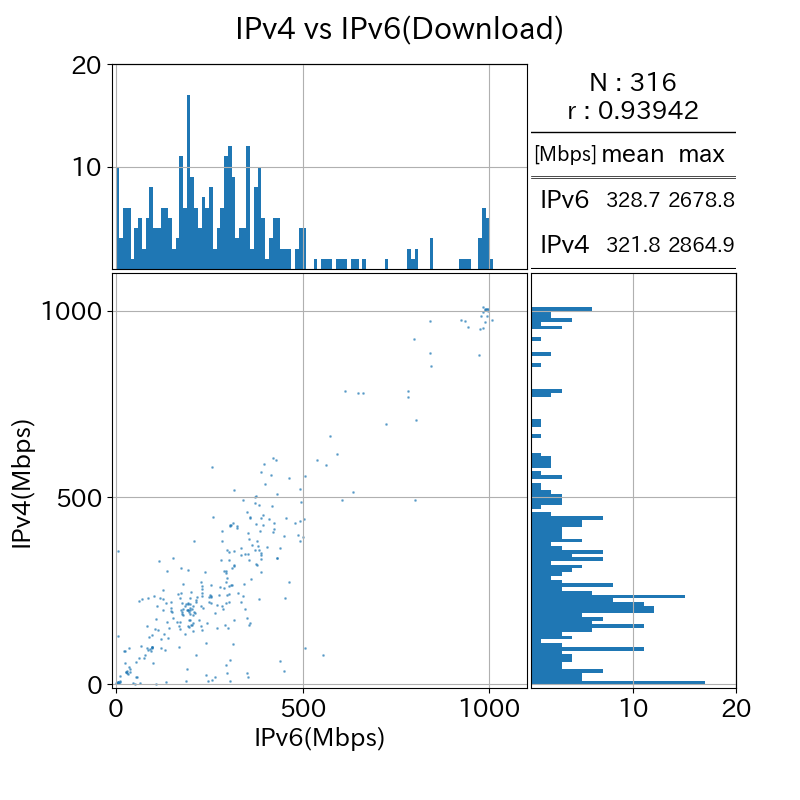
\includegraphics[width=0.8\textwidth]{fig/old_PPPoE_dl.png}
                \subcaption{IPv4/IPv6でPPPoEを使用した場合}
                \label{old_PPPoE_dl}
            \end{subfigure}
        \caption{(1)のダウンロードのスループット}
        \label{fig:old_connect_dl}
        \end{minipage}
        \hfill
        \begin{minipage}[t]{0.48\textwidth}
            \begin{subfigure}[b]{\textwidth}
                \centering
                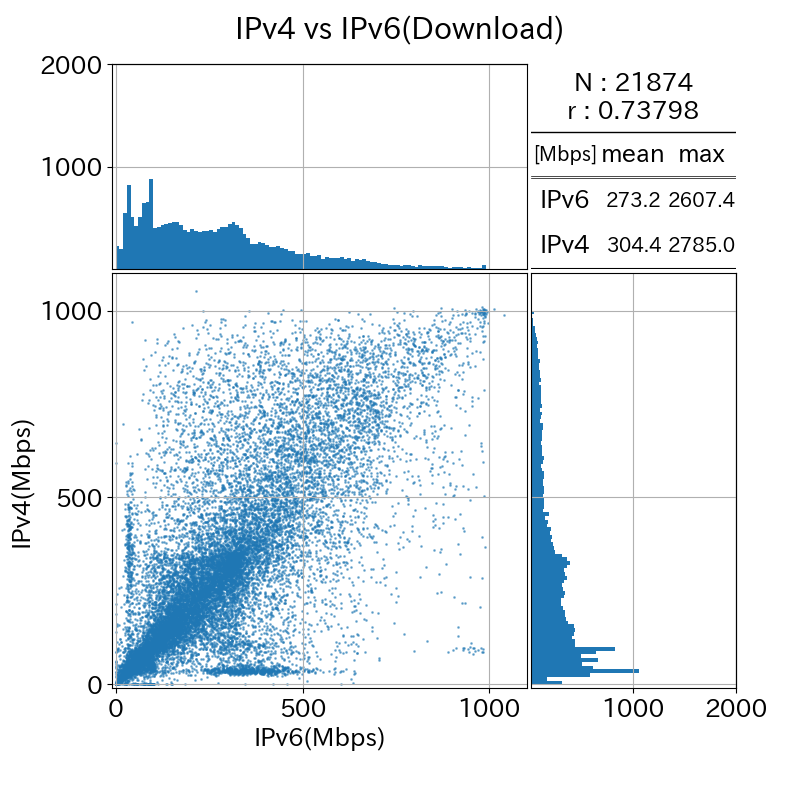
\includegraphics[width=0.8\textwidth]{fig/new_IPv4aaS_dl.png}
                \subcaption{IPv4/IPv6でIPoEを使用した場合}
                \label{new_IPv4aaS_dl}
            \end{subfigure}
            \begin{subfigure}[b]{\textwidth}
                \centering
                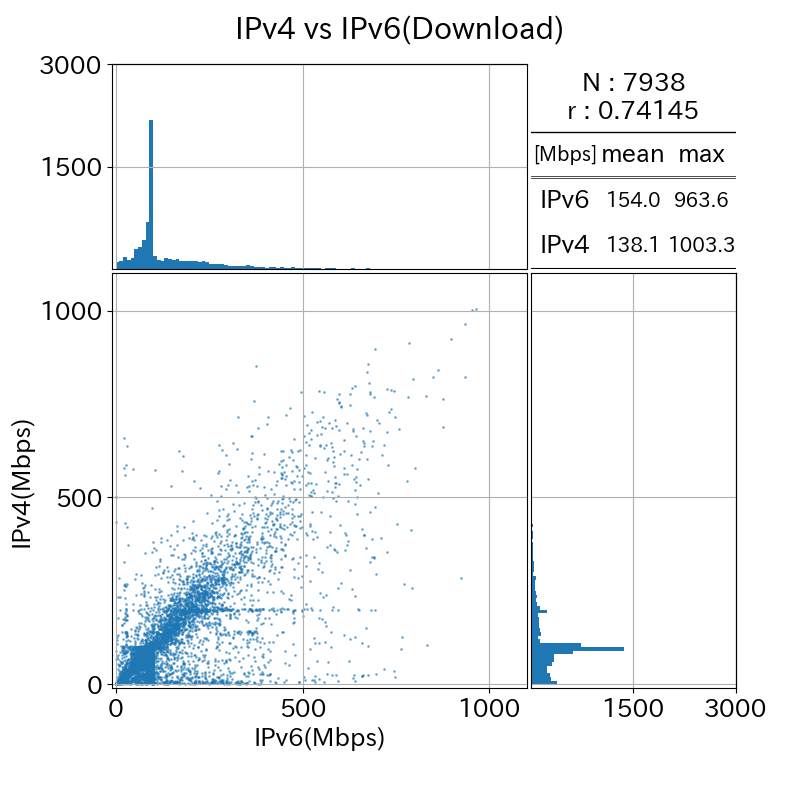
\includegraphics[width=0.8\textwidth]{fig/new_mix_dl.png}
                \subcaption{IPv4はPPPoE,IPv6はIPoEを使用した場合}
                \label{new_mix_dl}
            \end{subfigure}
            \begin{subfigure}[b]{\textwidth}
                \centering
                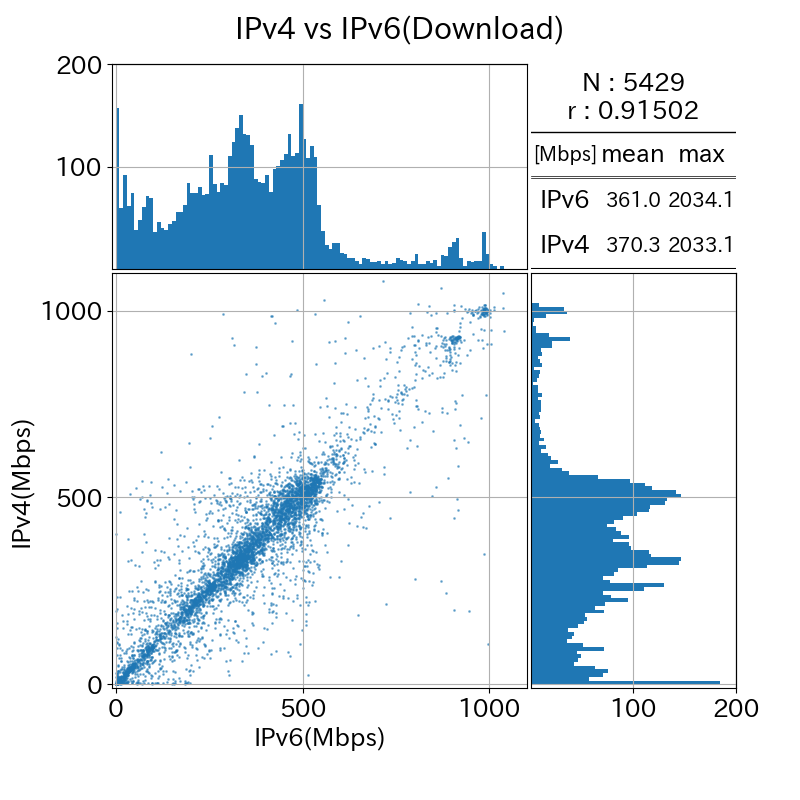
\includegraphics[width=0.8\textwidth]{fig/new_PPPoE_dl.png}
                \subcaption{IPv4/IPv6でPPPoEを使用した場合}
                \label{new_PPPoE_dl}
            \end{subfigure}
            \caption{(2)のダウンロードのスループット}
            \label{fig:new_connect_dl}
        \end{minipage}
    \end{center}
\end{figure}
\FloatBarrier

\begin{figure}[htbp]
    %\centering
    \begin{center}
        % 左側の図
        \begin{minipage}[t]{0.48\textwidth}
            \begin{center}
                \begin{subfigure}[b]{\textwidth}
                    \centering
                    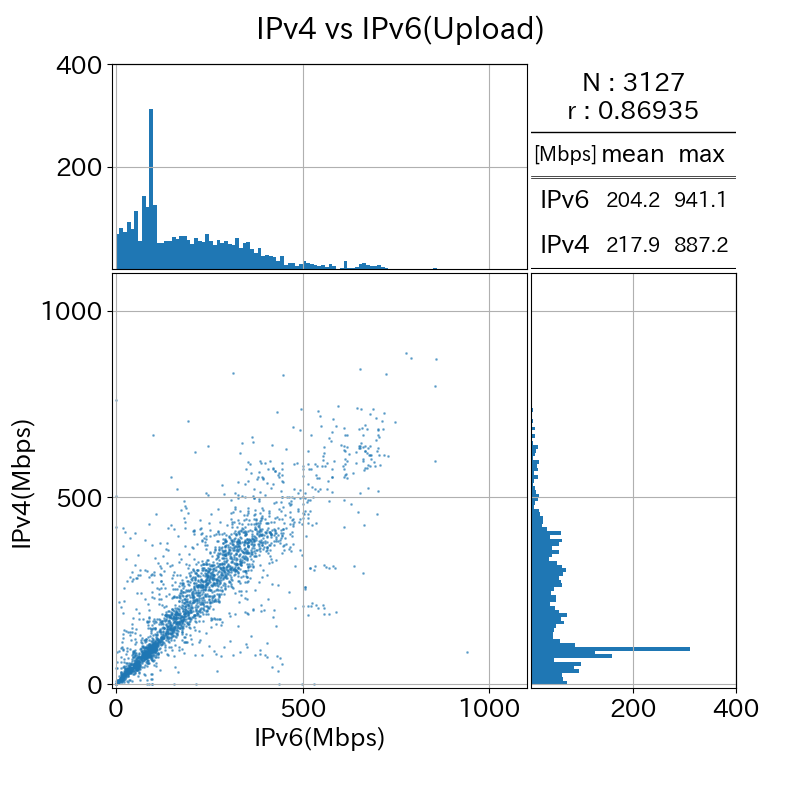
\includegraphics[width=0.8\textwidth]{fig/old_IPv4aaS_ul.png}
                    \subcaption{IPv4/IPv6でIPoEを使用した場合}
                    \label{old_IPv4aaS_ul}
                \end{subfigure}
                \begin{subfigure}[b]{\textwidth}
                    \centering
                    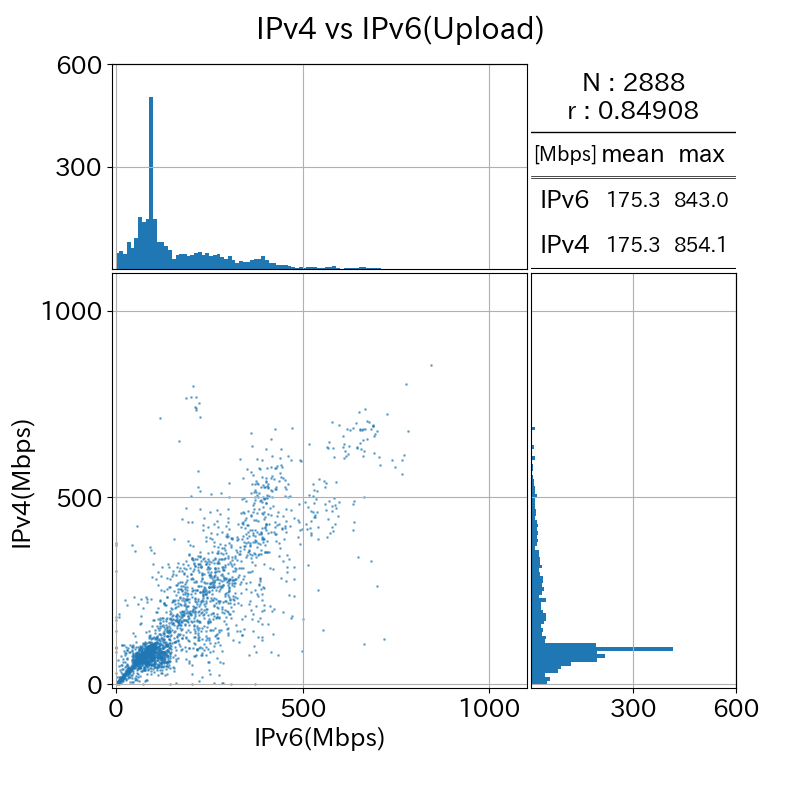
\includegraphics[width=0.8\textwidth]{fig/old_mix_ul.png}
                    \subcaption{IPv4はPPPoE,IPv6はIPoEを使用した場合}
                    \label{old_mix_ul}
                \end{subfigure}
                \begin{subfigure}[b]{\textwidth}
                    \centering
                    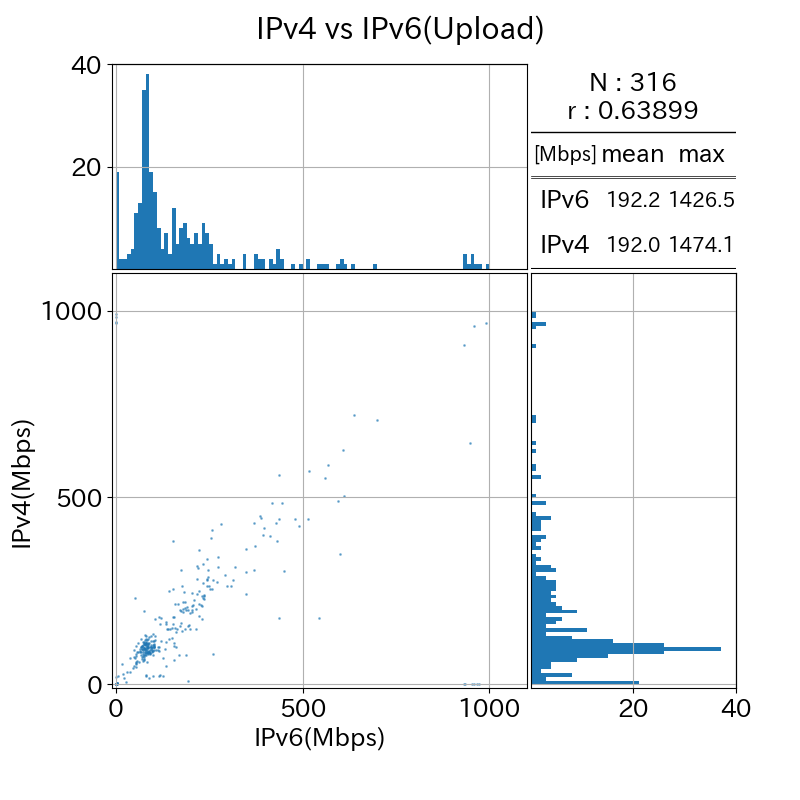
\includegraphics[width=0.8\textwidth]{fig/old_PPPoE_ul.png}
                    \subcaption{IPv4/IPv6でPPPoEを使用した場合}
                    \label{old_PPPoE_ul}
                \end{subfigure}
            \caption{(1)のアップロードのスループット}
            \label{fig:old_connect_ul}
            \end{center}
        \end{minipage}
        \hfill
        \begin{minipage}[t]{0.48\textwidth}
            \begin{subfigure}[b]{\textwidth}
                \centering
                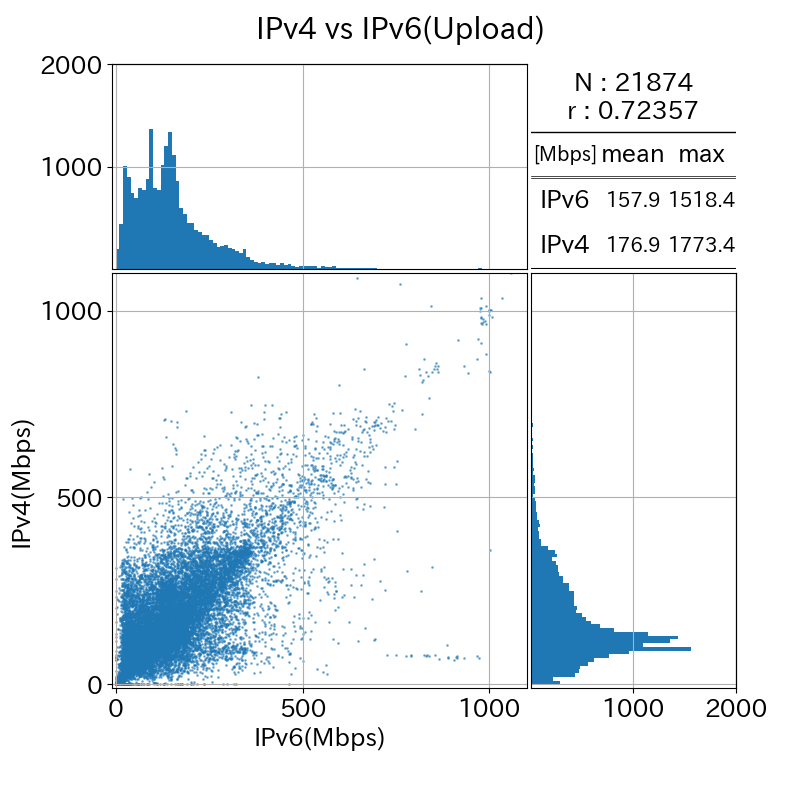
\includegraphics[width=0.8\textwidth]{fig/new_IPv4aaS_ul.png}
                \subcaption{IPv4/IPv6でIPoEを使用した場合}
                \label{new_IPv4aaS_ul}
            \end{subfigure}
            \begin{subfigure}[b]{\textwidth}
                \centering
                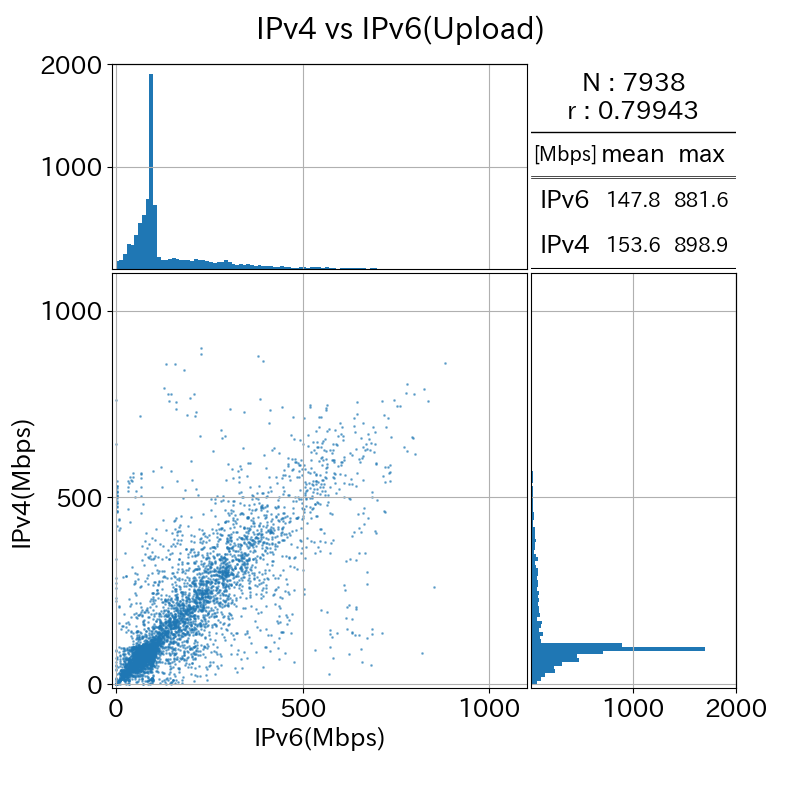
\includegraphics[width=0.8\textwidth]{fig/new_mix_ul.png}
                \subcaption{IPv4はPPPoE,IPv6はIPoEを使用した場合}
                \label{new_mix_ul}
            \end{subfigure}
            \begin{subfigure}[b]{\textwidth}
                \centering
                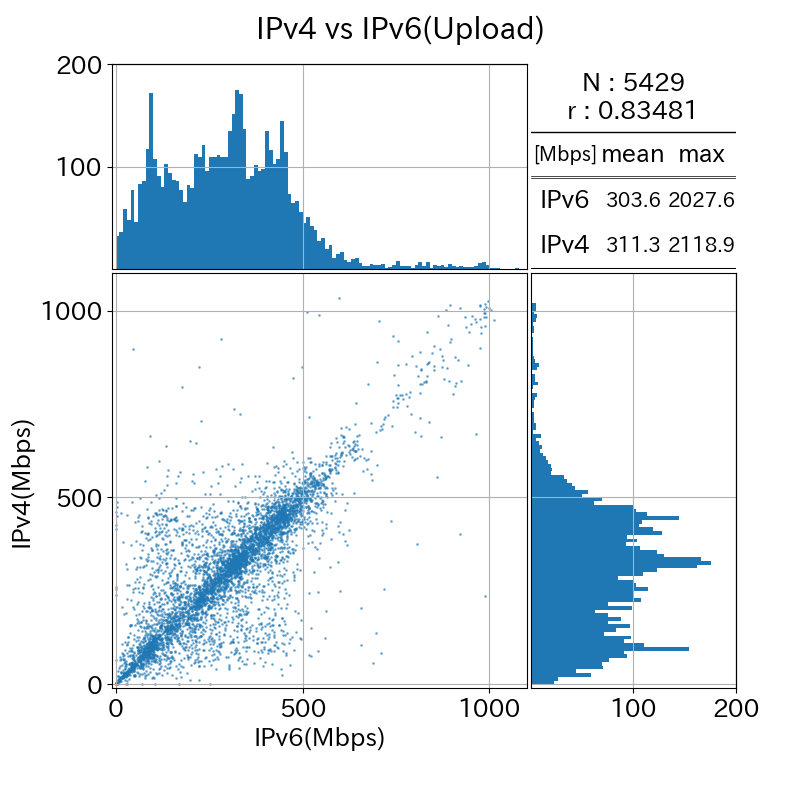
\includegraphics[width=0.8\textwidth]{fig/new_PPPoE_ul.png}
                \subcaption{IPv4/IPv6でPPPoEを使用した場合}
                \label{new_PPPoE_ul}
            \end{subfigure}
            \caption{(2)のアップロードのスループット}
            \label{fig:new_connect_ul}
        \end{minipage}
    \end{center}
\end{figure}
\FloatBarrier
%\end{comment}

%%%%%%%%%%%%%%%%%%%%%%%%%%%%%%%%%%%%%%%%%%%%%%%%%%%%%%%%%%%%%%%%%%%%%%%%%%
\section{RTTの調査}
\label{sec:rtt}
\cref{sec:throughput}と同様の手法を用いてRTTについて調査した.
\subsection{ISPの網によるRTTへの影響}
\cref{fig:old_isp_rtt,fig:new_isp_rtt}はそれぞれの期間のISPの網の違いによるRTTの比較を示す.\cref{old_sameISP_rtt,new_sameISP_rtt}は同じISPを使用した場合の結果で,\cref{old_diffISP_rtt,new_diffISP_rtt}は異なるISPを使用した場合の結果である.これらの間に振る舞いの違いは見られないことがわかった.

%%%%%%%%%%%%%%%%%%%%%%%%%%%%%%%%%%%%%%%%%%%%%%%%%%%%%%%%%%%%%%%%%%%%%%%%%%

\subsection{アクセス網の種類によるRTTへの影響}
\cref{fig:old_Line_rtt,fig:new_Line_rtt}はそれぞれの期間のアクセス網の種類によるRTTの比較を示す.\cref{old_FTTH_rtt,new_FTTH_rtt}がFTTHを使用した場合,\cref{old_CATV_rtt,new_CATV_rtt}はCATVを使用した場合,\cref{old_Mobile_rtt,new_Mobile_rtt}はMobileを使用した場合の結果である.FTTHとCATVを使用した場合のRTTはほぼ同じ振る舞いをしていると言える.一方,Mobileを使用した場合のRTTはFTTHやCATVに比べてRTTの平均値が大きい.平均値だけでなく,散布図の分布やヒストグラムのピークの場所からわかる.

%%%%%%%%%%%%%%%%%%%%%%%%%%%%%%%%%%%%%%%%%%%%%%%%%%%%%%%%%%%%%%%%%%%%%%%%%%
\subsection{インターネット接続方式によるRTTへの影響}
\cref{fig:old_connect_rtt,fig:new_connect_rtt}はそれぞれの期間のインターネット接続方式によるRTTの比較を示す.\cref{old_IPv4aaS_rtt,new_IPv4aaS_rtt}はIPv4/IPv6でIPoEを使用した場合,\cref{old_mix_rtt,new_mix_rtt}はIPv4はPPPoE,IPv6はIPoEを使用した場合,\cref{old_PPPoE_rtt,new_PPPoE_rtt}はIPv4/IPv6でPPPoEを使用した場合の結果である.これらの間も振る舞いの違いは見られないことがわかった.

%\begin{comment}
\begin{figure}[htbp]
    \begin{center}
        \begin{subfigure}[b]{0.49\textwidth}
            \centering
            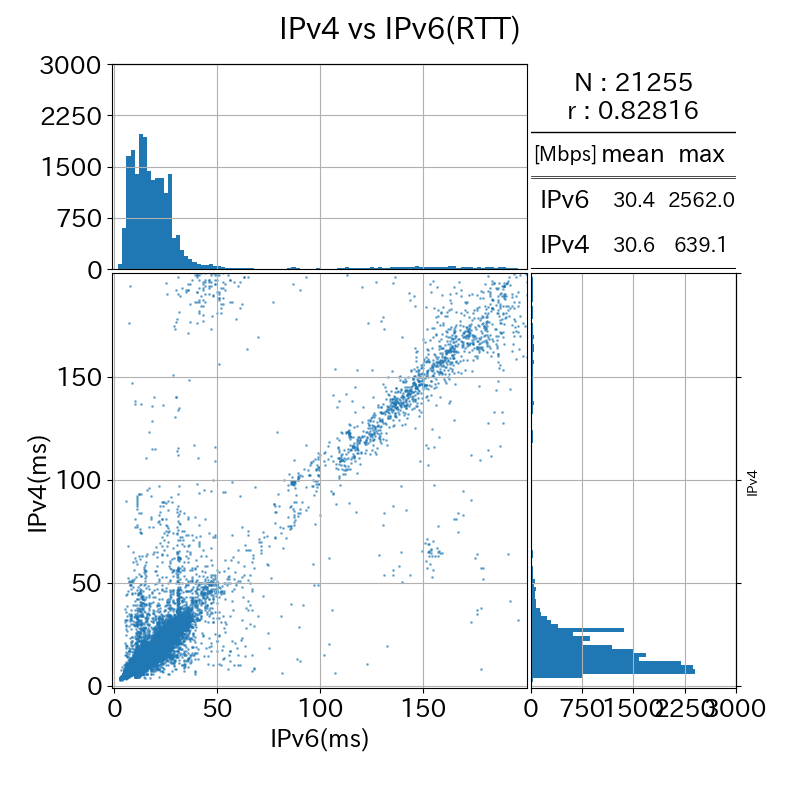
\includegraphics[width=1.0\textwidth]{fig/old_sameISP_rtt.png}
            \subcaption{同じISPを使用した場合}
            \label{old_sameISP_rtt}
        \end{subfigure}
        \begin{subfigure}[b]{0.49\textwidth}
            \centering
            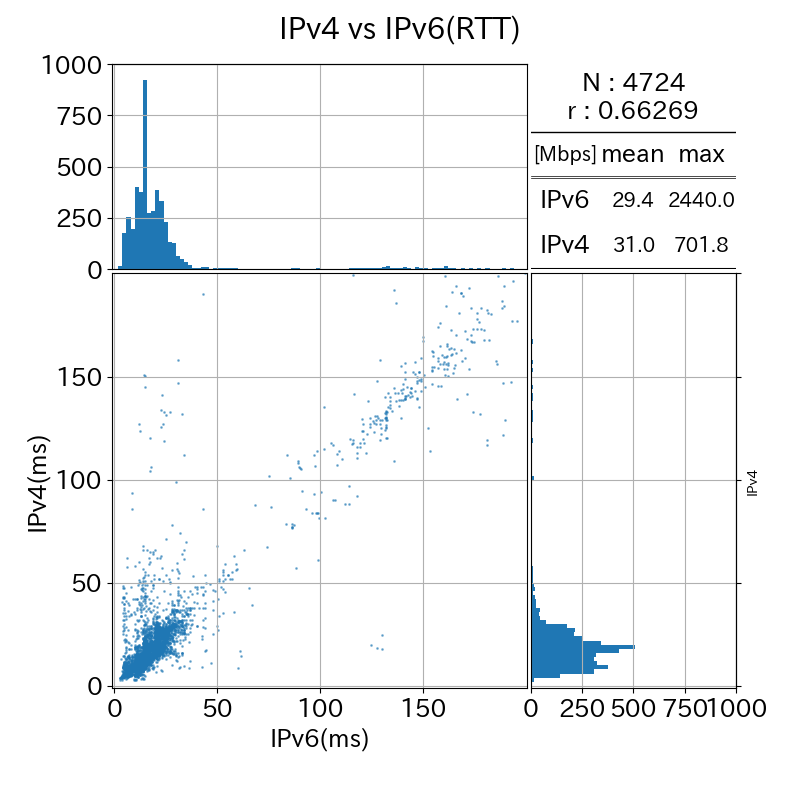
\includegraphics[width=1.0\textwidth]{fig/old_diffISP_rtt.png}
            \subcaption{異なるISPを使用した場合}
            \label{old_diffISP_rtt}
        \end{subfigure}
        \caption{{\bf 期間(1)}におけるRTT}
        \label{fig:old_isp_rtt}
    
        \begin{subfigure}[b]{0.49\textwidth}
            \centering
            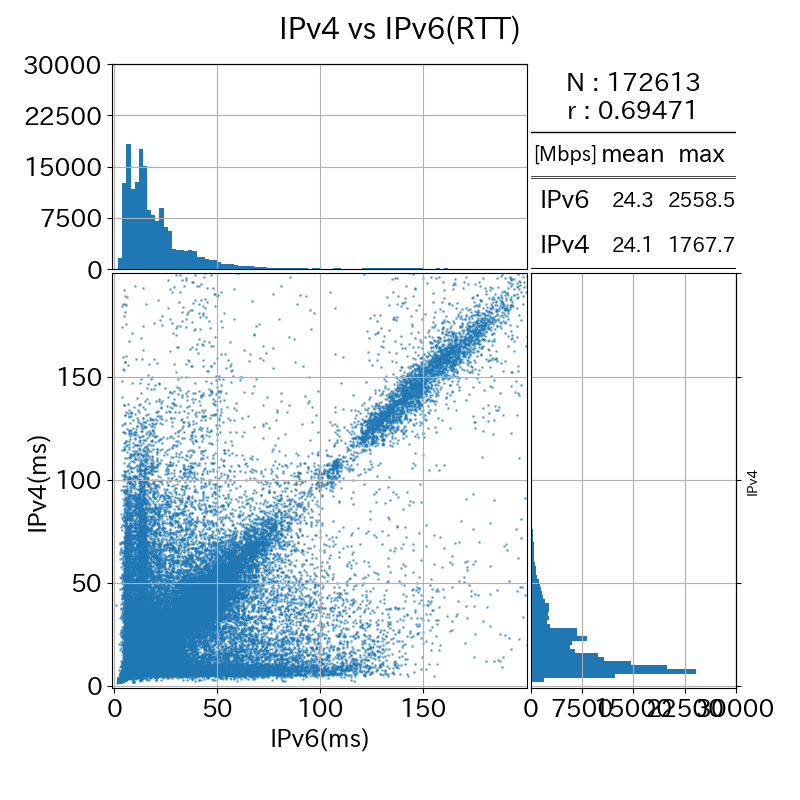
\includegraphics[width=1.0\textwidth]{fig/new_sameISP_rtt.png}
            \subcaption{同じISPを使用した場合}
            \label{new_sameISP_rtt}
        \end{subfigure}
        \begin{subfigure}[b]{0.49\textwidth}
            \centering
            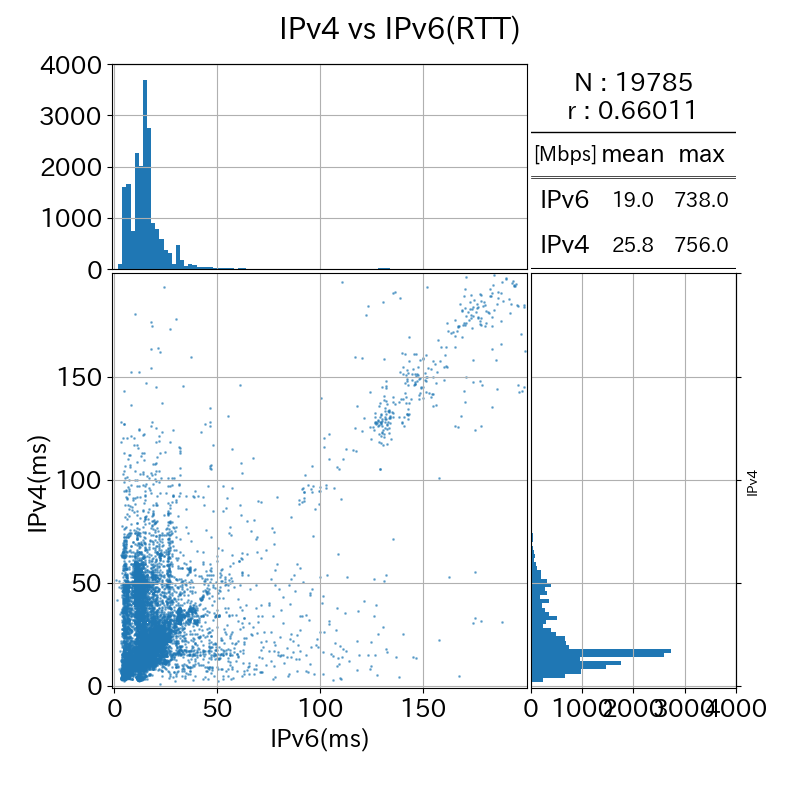
\includegraphics[width=1.0\textwidth]{fig/new_diffISP_rtt.png}
            \subcaption{異なるISPを使用した場合}
            \label{new_diffISP_rtt}
        \end{subfigure}
        \caption{{\bf 期間(2)}におけるRTT}
        \label{fig:new_isp_rtt}
    \end{center}
\end{figure}
\FloatBarrier
%\end{comment}

%\begin{comment}
\begin{figure}[htbp]
    %\centering
    \begin{center}
        % 左側の図
        \begin{minipage}[t]{0.48\textwidth}
            \begin{center}
                \begin{subfigure}[b]{\textwidth}
                    \centering
                    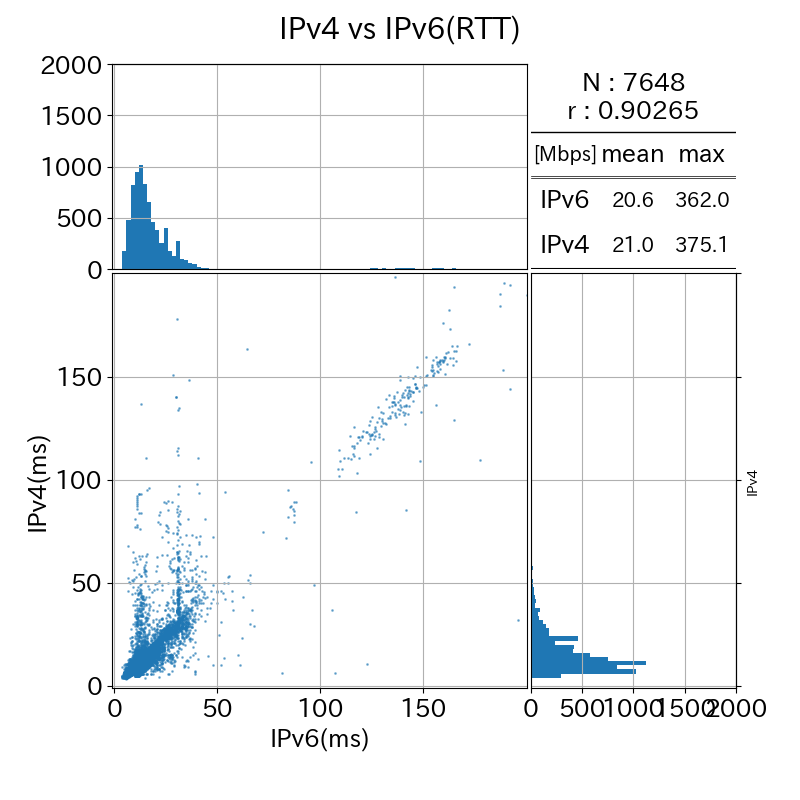
\includegraphics[width=0.85\textwidth]{fig/old_FTTH_rtt.png}
                    \subcaption{FTTHを使用した場合}
                    \label{old_FTTH_rtt}
                \end{subfigure}
                \begin{subfigure}[b]{\textwidth}
                    \centering
                    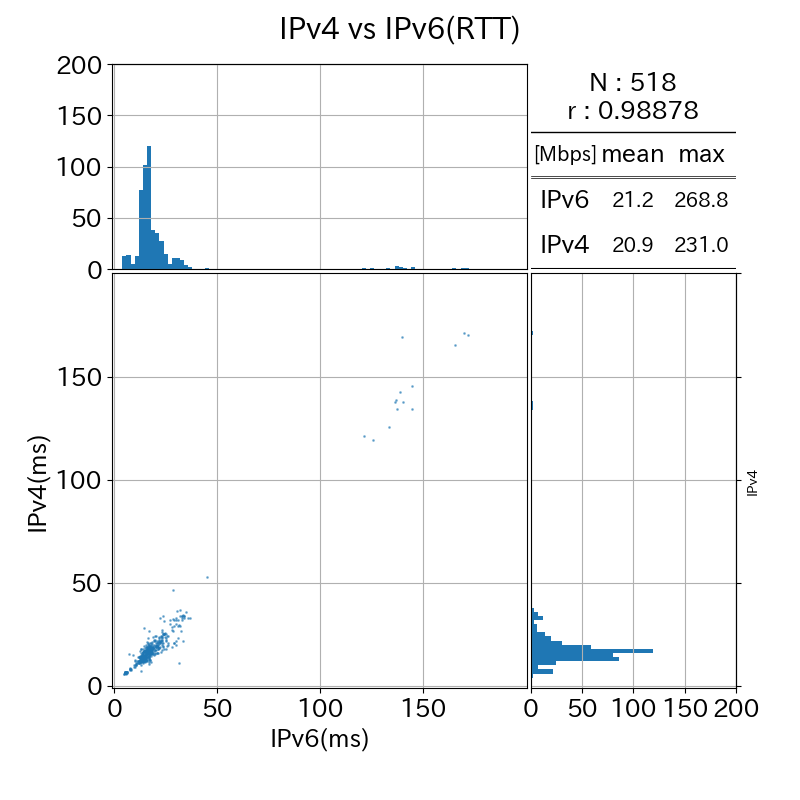
\includegraphics[width=0.85\textwidth]{fig/old_CATV_rtt.png}
                    \subcaption{CATVを使用した場合}
                    \label{old_CATV_rtt}
                \end{subfigure}
                \begin{subfigure}[b]{\textwidth}
                    \centering
                    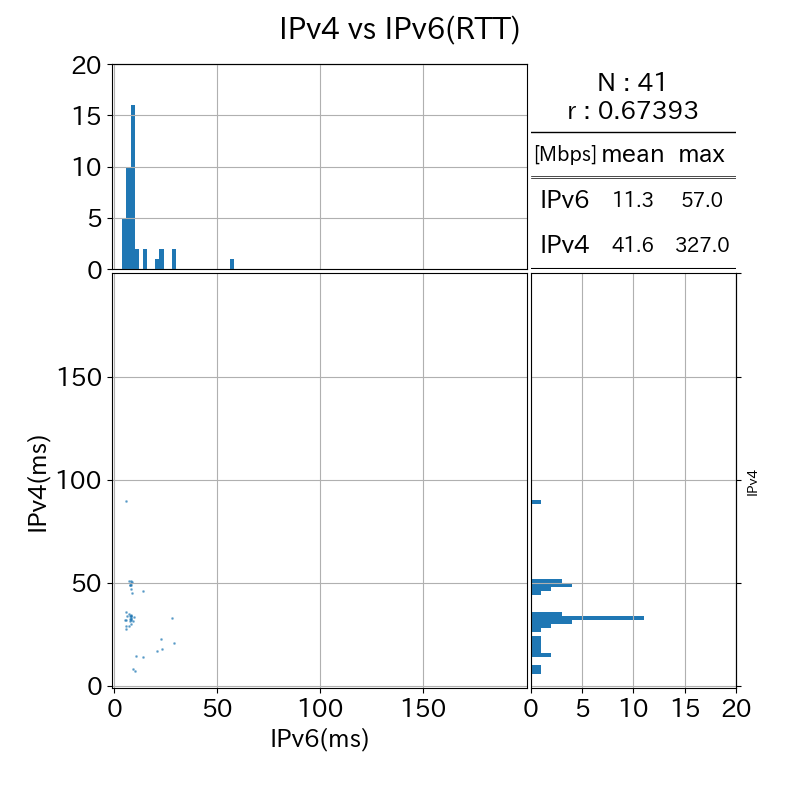
\includegraphics[width=0.85\textwidth]{fig/old_Mobile_rtt.png}
                    \subcaption{Mobileを使用した場合}
                    \label{old_Mobile_rtt}
                \end{subfigure}
            \caption{{\bf 期間(1)}におけるRTT}
            \label{fig:old_Line_rtt}
            \end{center}
        \end{minipage}
        \hfill
        \begin{minipage}[t]{0.48\textwidth}
            \begin{subfigure}[b]{\textwidth}
                \centering
                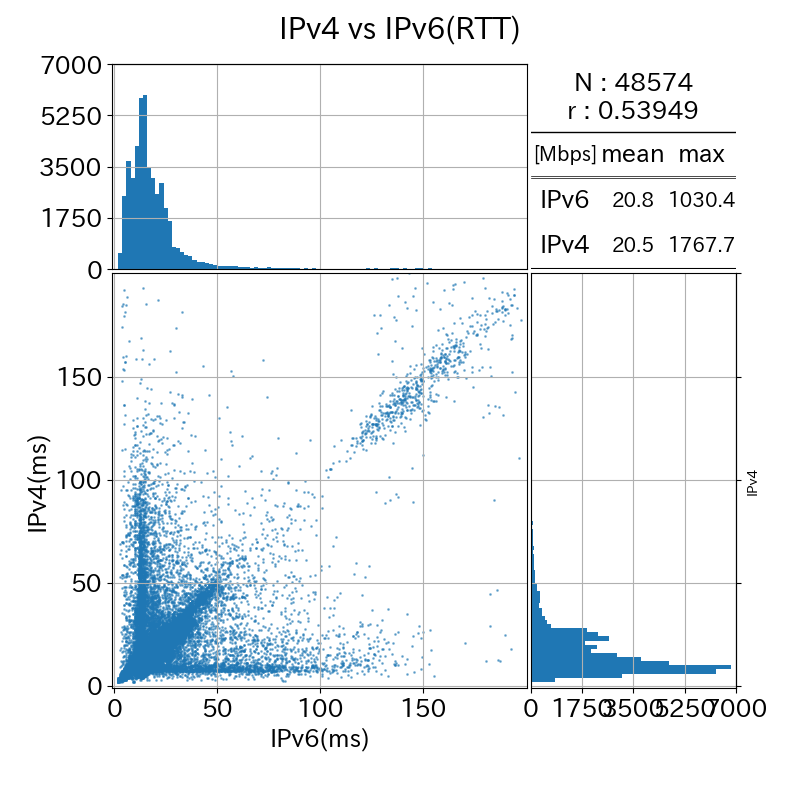
\includegraphics[width=0.85\textwidth]{fig/new_FTTH_rtt.png}
                \subcaption{FTTHを使用した場合}
                \label{new_FTTH_rtt}
            \end{subfigure}
            \begin{subfigure}[b]{\textwidth}
                \centering
                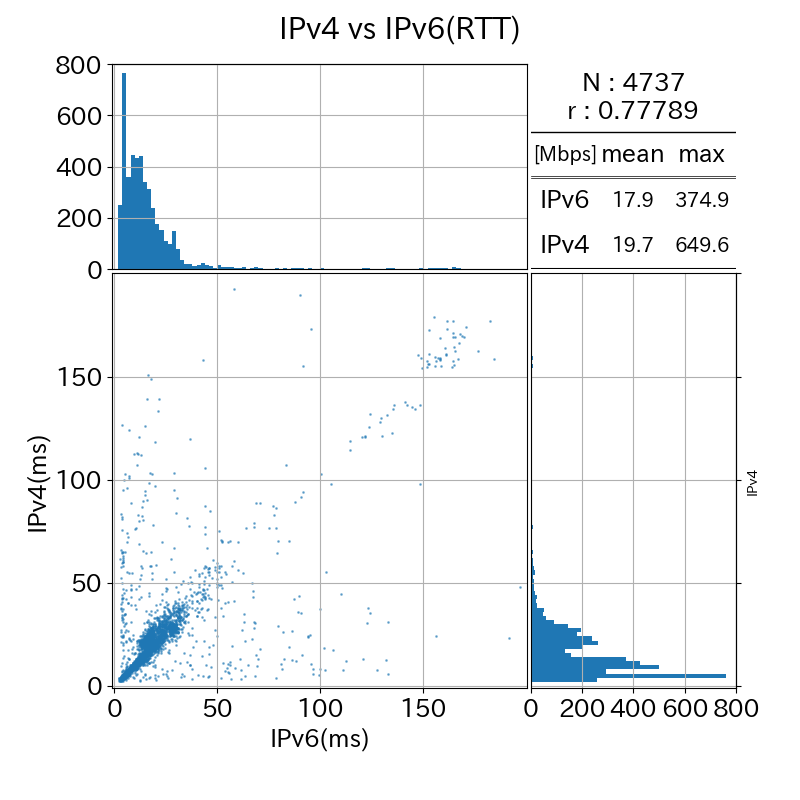
\includegraphics[width=0.85\textwidth]{fig/new_CATV_rtt.png}
                \subcaption{CATVを使用した場合}
                \label{new_CATV_rtt}
            \end{subfigure}
            \begin{subfigure}[b]{\textwidth}
                \centering
                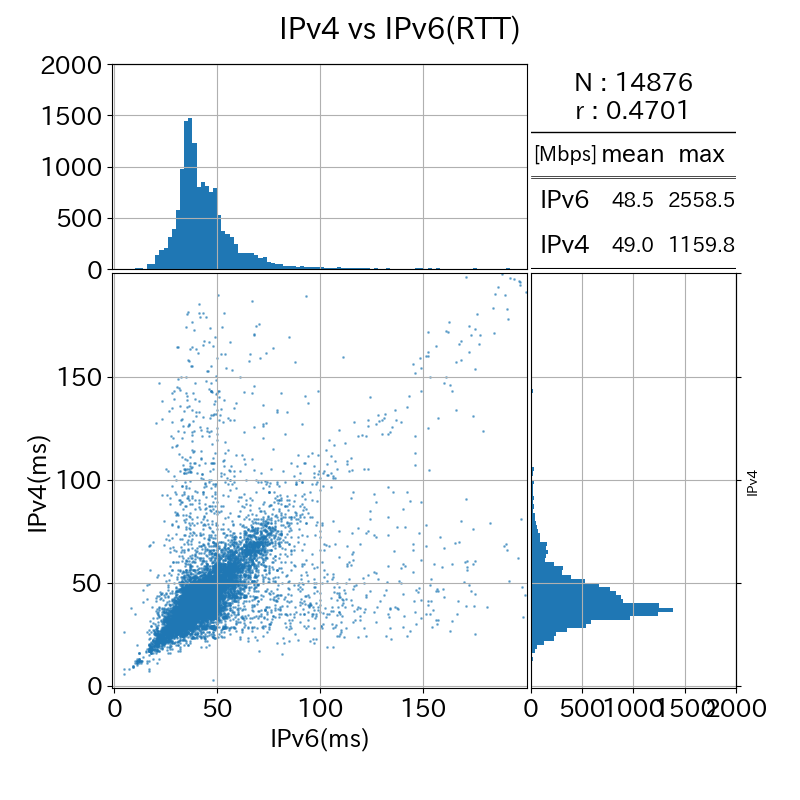
\includegraphics[width=0.85\textwidth]{fig/new_Mobile_rtt.png}
                \subcaption{Mobileを使用した場合}
                \label{new_Mobile_rtt}
            \end{subfigure}
            \caption{{\bf 期間(2)}におけるRTT}
            \label{fig:new_Line_rtt}
        \end{minipage}
    \end{center}
\end{figure}
\FloatBarrier
%\end{comment}

%\begin{comment}
\begin{figure}
    %\centering
    \begin{center}
        % 左側の図
        \begin{minipage}[t]{0.48\textwidth}
            \begin{subfigure}[b]{\textwidth}
                \centering
                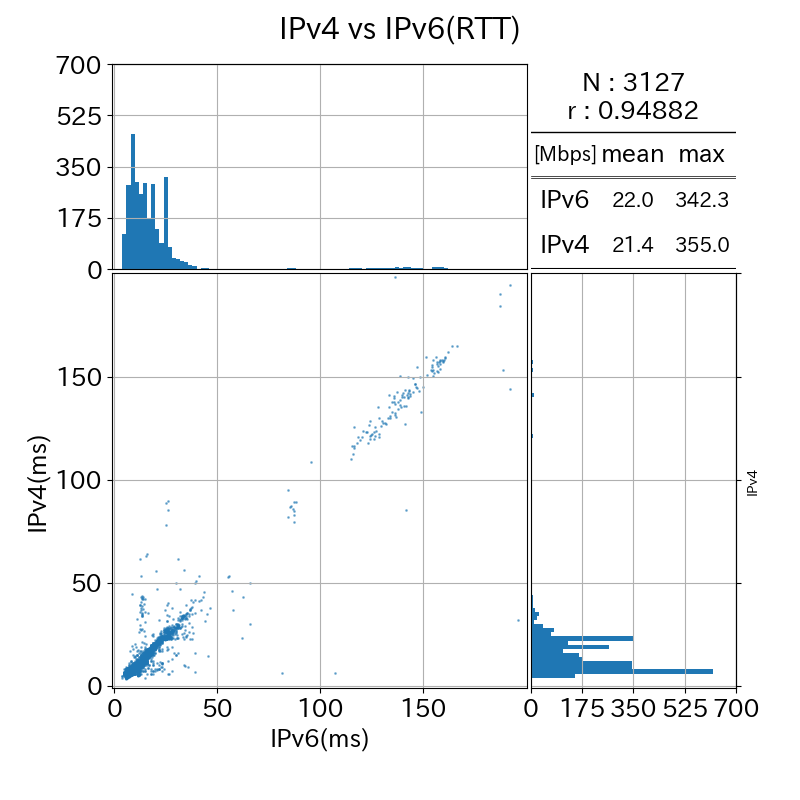
\includegraphics[width=0.85\textwidth]{fig/old_IPv4aaS_rtt.png}
                \subcaption{IPv4/IPv6でIPoEを使用した場合}
                \label{old_IPv4aaS_rtt}
            \end{subfigure}
            \begin{subfigure}[b]{\textwidth}
                \centering
                \includegraphics[width=0.85\textwidth]{fig/old_mix_rtt.png}
                \subcaption{IPv4はPPPoE,IPv6はIPoEを\\使用した場合}
                \label{old_mix_rtt}
            \end{subfigure}
            \begin{subfigure}[b]{\textwidth}
                \centering
                \includegraphics[width=0.85\textwidth]{fig/old_PPPoE_rtt.png}
                \subcaption{IPv4/IPv6でPPPoEを使用した場合}
                \label{old_PPPoE_rtt}
            \end{subfigure}
            \caption{{\bf 期間(1)}におけるRTT}
            \label{fig:old_connect_rtt}
        \end{minipage}
        \hfill
        \begin{minipage}[t]{0.48\textwidth}
            \begin{subfigure}[b]{\textwidth}
                \centering
                \includegraphics[width=0.85\textwidth]{fig/new_IPv4aaS_rtt.png}
                \subcaption{IPv4/IPv6でIPoEを使用した場合}
                \label{new_IPv4aaS_rtt}
            \end{subfigure}
            \begin{subfigure}[b]{\textwidth}
                \centering
                \includegraphics[width=0.85\textwidth]{fig/new_mix_rtt.png}
                \subcaption{IPv4はPPPoE,IPv6はIPoEを\\使用した場合}
                \label{new_mix_rtt}
            \end{subfigure}
            \begin{subfigure}[b]{\textwidth}
                \centering
                \includegraphics[width=0.85\textwidth]{fig/new_PPPoE_rtt.png}
                \subcaption{IPv4/IPv6でPPPoEを使用した場合}
                \label{new_PPPoE_rtt}
            \end{subfigure}
            \caption{{\bf 期間(2)}におけるRTT}
            \label{fig:new_connect_rtt}
        \end{minipage}
    \end{center}
\end{figure}
\FloatBarrier
%\end{comment}

%%%%%%%%%%%%%%%%%%%%%%%%%%%%%%%%%%%%%%%%%%%%%%%%%%%%%%%%%%%%%%%%%%%%%%%%%%
\section{調査のまとめ}
本章ではアクセス環境による通信品質への影響を調査した.スループットにはアクセス環境によって異なる振る舞いが見られた.ISP網内の通信環境や,アクセス網の種類の限界,インターネット接続方式の組み合わせの違いなどさまざまな要因でスループットに影響があるため,分析時には慎重な判断が必要である.CATVのように時期によって振る舞いが変化場合や,インターネット接続方式の違いのように他の要因も考えられる場合もあることから,引き続き調査をする必要があることがわかった.
一方,RTTについてはアクセス環境による振る舞いの違いはほとんど見られなかった.RTTはアクセス環境の種類よりも,地域による影響が大きいと予想される.先行研究\cite{nasu}では物理的距離だけでなくISP内のトポロジーやISP間の経路による影響が確認されている.これらの要因がスピードテストサイトの計測ログにも同様の傾向が見られるか調査するために,計測ログに付与する情報を増やし新たなアクセス環境を定義して調査する必要がある.

これらの結果から,スピードテストサイトの計測ログを使用して通信品質の分析をするとき,対象とアクセス環境のデータを抽出してから分析を行うことが重要であることがわかった.

\chapter{可視化システム}
\label{chap:system}
\cref{chap:access}からアクセス環境によってスループットに差が生じることがわかった.しかし,アクセス環境の影響についてユーザーに伝えているスピードテストサイトがない.そこで,本章ではアクセス環境の影響をユーザーに伝えるための可視化システム,iNoniusスピードテスト統計情報可視化システムについて述べる.

\section{システムの概要}
\subsection{システムの構成}
\cref{fig:system_image} にシステム構成を示す.システムは,iNonius統計情報可視化システムサーバーとiNonius Speed Testサーバー,クライアント端末から構成される.iNonius統計情報可視化システムサーバーには,Webサーバーコンテナと画像生成コンテナ,データ処理コンテナ,可視化システム用DBが存在する.データ処理コンテナはiNonius スピードテストサーバーから毎月の計測ログを取得し,アクセス環境ごとに最大値,最小値,中央値,四分位範囲,平均値からなる統計情報を算出し,統計量記録用テーブルに保存する.統計量記録用テーブルから 1 年分の統計量を取得して,表示用の画像を作成して,グラフ画像記録用テーブルにバイナリデータとして保存する.クライアントからのアクセス環境ごとの集計結果の要求を Web サーバーコンテナを受け取ると画像生成コンテナを経由して,グラフ画像記録用テーブルからバイナリデータを取得後,要求に対応する 1 年分の集計結果のグラフを画像(JPEG) ファイルとしてクライアントに返す.\cref{fig:system_v6_catv_dl}はアクセス回線が CATV の場合の IPv6 のダウンロードスループットのグラフである.可視化サイトにはアクセス環境ごとに IPv4 と IPv6,ダウンロードとアップロードのスループットをそれぞれ示す 4 つのグラフが表示される.

%%\begin{comment}
\begin{figure}[htbp]
    \centering
    \vspace{40pt} % Adjust the space between the figures
    \includegraphics[width=1.0\textwidth]{fig/system_image.png}
    \caption{iNonius スピードテストサイト統計情報可視化システムのシステム構成}
    \label{fig:system_image}
    \vspace{20pt} % Adjust the space between the figures
    \includegraphics[width=1.0\textwidth]{fig/box_image.jpg}
    \caption{CATV回線のダウンロード速度のグラフ}
    \label{fig:system_v6_catv_dl}
    \vspace{40pt} % Adjust the space between the figures
\end{figure}
\FloatBarrier
%%\end{comment}

\subsection{データ処理コンテナ}
データ処理コンテナ内で実行されるデータ処理とグラフ画像の作成フローを\cref{fig:graph_flow}に示す.iNonius Speed Testのデータベースから毎月の計測ログを取得し,前処理として外れ値を含む計測ログを除外する.このとき,外れ値として除外されるのは欠損値を含むデータとスループットの計測結果が小数第2位まで0を記録するデータである.欠損値を含むデータは統計情報を算出するときに,エラーの原因になるため除外する.スループットの計測結果が小数第2位まで0を記録するデータは計測が完了していない不完全なデータと推定されるため,異常値として除外している.アクセス環境の分類は,\cref{label:accesstype}と同様の手法を用いて分類している.アクセス環境ごとに最大値,最小値,中央値,四分位範囲,平均値からなる統計情報を算出し統計量記録用テーブルを更新する.統計量記録用テーブルには,アクセス環境の種類とデータの期間,アップロードとダウロードの判定フラグ,IPv4/IPv6の判定フラグ,統計情報が記録される.統計量記録用テーブルから 1 年分の統計量を取得して\cref{fig:system_v6_catv_dl}のような表示用のグラフ画像を作成する.グラフには箱ひげ図を用いている.箱ひげ図を用いることで,計測ログの分布を可視化できることを目的としている.また,総務省が発表している通信品質の調査に関するガイドライン\cite{mobile_guideline}\cite{bb_guideline}でも採用されており,通信品質を可視化するのに適していると考えられる.画像のバイナリデータをグラフ画像記録用テーブルにアクセス環境の種類とデータの期間,アップロードとダウロードの判定フラグ,IPv4/IPv6の判定フラグとともに保存する.
一連の処理を月次で実行しているため,毎月の計測ログから統計情報を算出し,グラフ画像を作成している.

%%\begin{comment}
\begin{figure}[htbp]
    \centering
    \includegraphics[width=0.8\textwidth]{fig/graph_flow.png}
    \caption{データ処理コンテナの処理フロー}
    \label{fig:graph_flow}
\end{figure}
\FloatBarrier
%%\end{comment}

\subsection{画像生成コンテナ}
画像生成コンテナはクライアントからのアクセス環境ごとの集計結果の要求を受け取り,グラフ画像記録用テーブルからバイナリデータを取得して,要求に対応する 1 年分の集計結果のグラフを画像(JPEG)ファイルとしてクライアントに返すコンテナである.Webサーバーコンテナと画像生成コンテナの処理フローをそれぞれ\cref{fig:web_flow},\cref{fig:fig_flow}に,シーケンス図を\cref{fig:sequence}に示す.
Webサーバーコンテナはクライアントからのリクエストを受け取り,画像生成コンテナにアクセス環境に基づいたグラフ画像の生成をリクエストする.画像生成コンテナはグラフ画像記録用テーブルから必要なデータを取得し,グラフ画像を生成して一時ファイルとしてホスト上に保存する.その後,Webサーバーコンテナに一時ファイルのアドレスを返し,Webサーバーコンテナはクライアントにグラフ画像を表示する.

%%\begin{comment}
\begin{figure}[htbp]
    \centering
    \includegraphics[width=0.6\textwidth]{fig/web_flow.png}
    \caption{Webサーバーコンテナの処理フロー}
    \label{fig:web_flow}
\end{figure}
\FloatBarrier
%%\end{comment}

%%\begin{comment}
\begin{figure}[htbp]
    \centering
    \includegraphics[width=1.0\textwidth]{fig/fig_flow.png}
    \caption{画像生成コンテナの処理フロー}
    \label{fig:fig_flow}
\end{figure}
\FloatBarrier
%%\end{comment}

%%\begin{comment}
\begin{figure}[htbp]
    \centering
    \includegraphics[width=1.0\textwidth]{fig/sequence.png}
    \caption{シーケンス図}
    \label{fig:sequence}
\end{figure}
\FloatBarrier
%%\end{comment}

\subsection{開発環境}
開発システムのホストの開発環境を\cref{tab:host}に,Webサーバーコンテナの開発環境を\cref{tab:webserver}に,画像生成コンテナの開発環境を\cref{tab:image}に,データ処理コンテナの開発環境を\cref{tab:dataprocessing}に,データベースコンテナの開発環境を\cref{tab:database}に示す.

\begin{table}
    \centering
    \caption{ホストの開発環境}
    \label{tab:host}
    \begin{tabular}{cc}
        \hline
        項目 & 説明 \\
        \hline \hline
        OS & Ubuntu Ubuntu 22.04.5 LTS \\
        カーネル & 5.15.0-125-generic \\
        CPU & Inter(R) Core(TM) i7-9700 CPU @ 3.00GHz \\
        メモリ & 15GB \\
        Docker & Docker version 27.2.0, build 3ab4256 \\
        \hline
    \end{tabular}
\end{table}

\begin{table}
    \centering
    \caption{Webサーバーコンテナの開発環境}
    \label{tab:webserver}
    \begin{tabular}{cc}
        \hline
        項目 & 説明 \\
        \hline \hline
        OS & Alpine Linux v3.20 \\
        \hline
        nginx & nginx/1.27.2 \\
        \hline
        \end{tabular}
\end{table}

\begin{table}
    \centering
    \caption{画像生成コンテナの開発環境}
    \label{tab:image}
    \begin{tabular}{cc}
        \hline
        項目 & 説明 \\
        \hline \hline
        OS & Debian GNU/Linux 12 (bookworm) \\
        \hline
        Python & Python 3.9.20 \\
        \hline
        Flask & 3.0.3 \\
        \hline
        Flask-Cors & 5.0.0 \\
        \hline
        PyMySQL & 1.1.1 \\
        \hline
        SQLAlchemy & 2.0.36 \\
        \hline
    \end{tabular}
\end{table}

\begin{table}
    \centering
    \caption{データ処理コンテナの開発環境}
    \label{tab:dataprocessing}
    \begin{tabular}{cc}
        \hline
        項目 & 説明 \\
        \hline \hline
        OS & Debian GNU/Linux 12 (bookworm) \\
        \hline
        Python & Python 3.9.20 \\
        \hline
        PyMySQL & 1.1.1 \\
        \hline
        SQLAlchemy & 2.0.36 \\
        \hline
        matplotlib & 3.9.2 \\
        \hline
        numpy & 2.1.2 \\
        \hline
        pandas & 2.2.3 \\
        \hline
    \end{tabular}
\end{table}

\begin{table}
    \centering
    \caption{データベースコンテナの開発環境}
    \label{tab:database}
    \begin{tabular}{cc}
        \hline
        項目 & 説明 \\
        \hline \hline
        OS & Ubuntu 24.04.1 LTS \\
        \hline
        MariaDB & mariadb from 11.5.2-MariaDB \\
        \hline
        \end{tabular}
\end{table}

\section{システムの評価}
\subsection{ユーザーアンケート}
本システムはWebサイトとして\url{https://inonius.v6.netsci.info.hiroshima-cu.ac.jp/}で公開している.このサイトを利用したユーザーにアンケートを実施したアンケートをもとに評価を行う.
アンケートの設問を\cref{tab:questionnaire}に示す.設問は全部で 10 問あり,そのうちQ1からQ4は,本サイトを利用してもらうための質問であるため,それらは評価から除外してQ5からQ10について評価を行う.
Q5からQ7の回答を\cref{fig:Q5}から\ref{fig:Q7}に示す.
%\cref{tab:questionnaire}

\begin{table}[htbp]
    \centering
    \caption{アンケート項目}
    \begin{tabular}{lll}
        \hline
        番号 & 質問 & 回答方法 \\
        \hline \hline
        \vspace{10pt}
        Q1.&
        \begin{tabular}{l}
            普段,インターネットを使用しているときの\\通信品質の満足度をお答えください.\\
        \end{tabular}& 5段階評価\\
        \vspace{10pt}
        Q2.&
        \begin{tabular}{l}
            普段のインターネットを使用しているときの\\体感の通信品質と,iNoniusスピードテストの\\計測結果を比較したときどちらが上回っていますか?\\
        \end{tabular}& 5段階評価\\
        \vspace{10pt}
        Q3-1.&
        \begin{tabular}{l}
            本サイトの統計情報のうちあなたと同じアクセス環境の\\統計情報の直近1カ月の中央値とiNoniusスピードテストでの\\計測結果を直近比較したとき,どちらが速いですか?\\
        \end{tabular}& 5段階評価\\
        \vspace{10pt}
        Q3-2.&
        \begin{tabular}{l}
            本サイトの統計情報のうちあなたと異なるアクセス環境の\\統計情報の直近1カ月の中央値ととiNoniusスピードテストでの\\計測結果を直近比較したとき,どちらが速いですか?\\
        \end{tabular}& 5段階評価\\
        \vspace{10pt}
        Q4.&
        \begin{tabular}{l}
            本サイトの統計情報とiNoniusスピードテストの計測結果を\\比較して,ご自身の通信環境を見直そうと思いましたか?\\
        \end{tabular}& 4段階評価\\
        \vspace{10pt}
        Q5.&
        \begin{tabular}{l}
            iNoniusスピードテストの統計情報を可視化できることに\\意義を感じますか.\\
        \end{tabular}& 5段階評価\\
        \vspace{10pt}
        Q6.&
        \begin{tabular}{l}
            アクセス環境別の統計情報と計測結果を比較することに\\意義を感じたか.\\
        \end{tabular}& 5段階評価\\
        \vspace{10pt}
        Q7.&
        \begin{tabular}{l}
            本サイトで使用しているグラフ(箱ひげ図)の表現は\\適切だと思いますか.\\
        \end{tabular}& 5段階評価\\
        \vspace{10pt}
        Q8.&
        \begin{tabular}{l}
            上記の質問で「そう思わない」,「あまりそう思わない」と\\回答された方は,なぜそう思われたか,また改善案を\\教えてください.\\
        \end{tabular}& 自由記述\\
        \vspace{10pt}
        Q9.&
        \begin{tabular}{l}
            現在,アクセス環境によるスピードテストサイトでの\\計測に対する影響は調査を続けております.\\本サイトで定義しているアクセス環境以外に,\\調査してほしい条件などありましたらご意見ください.\\
        \end{tabular}& 自由記述\\
        \vspace{10pt}
        Q10.&
        \begin{tabular}{l}
            その他に本サイト並びに研究について自由にご意見ください.\\
        \end{tabular}& 自由記述\\
        \hline
    \end{tabular}
    \label{tab:questionnaire}
\end{table}
\FloatBarrier

Q5の回答から統計情報を可視化することは多くのユーザーが肯定来な回答をしているため,必要とされていることがわかる.一方で,Q6の回答からアクセス環境別の統計情報と計測結果を比較することに意義を感じるユーザーは全体の約70\%とQ5に比べて少ない.Q9で本サイトで示しているアクセス環境以外に調査してほしいアクセス環境を尋ねたところ,アクセス網の利用用途による違い,地理的な違い,アクセス網の種類を増やすことなどが挙げられた.公開したシステムではユーザーが知りたいようなアクセス環境を示すことができていないため,肯定的な意見が少ないと考えられる.定義しているアクセス環境は計測ログに含まれる情報から選択しているため,ユーザーが知りたいアクセス環境を示すことができていない.今後はさまざまな情報を計測ログに付与してユーザーに必要とされるアクセス環境を示すことができるようにする必要がある.

Q7のグラフの表現についても肯定的な意見が全体の約70\%である.Q7で「あまりそう思わない」「そう思わない」と回答したユーザーにQ8でなぜそう思ったかを自由記述で尋ねた.グラフのスケールの調整ができず比較が難しい,データの分布に関する情報が欲しい,という意見が挙がっている.本システムではグラフは画像で表示しているため,ユーザーはインタラクティブにグラフを操作することができず,比較が難しい.\cref{fig:bad_boxplot}に箱ひげ図の例を示す.この図はFTTH回線のダウンロード速度の箱ひげ図である.この図の,2023-12と2024-01の箱ひげ図は最小値と中央値,第1四分位数が重なっているように見えるため,比較することが難しい場合が考えられる.データの分布に関しては,箱ひげ図は第1四分位数,中央値,第3四分位数,最小値,最大値を表現しているため,データの分布に関する情報が得られると考えていたが,箱ひげ図はデータの分布を正確に表現することが難しい.スループットの計測結果は正規分布ではないため,データのボリューム層がどこにあるかを知るためには他の情報も必要である.今後はユーザーがインタラクティブにグラフを操作できるようにすることで,比較が容易になるようにする必要がある.また,データの分布に関する情報を示すために他のグラフを併用することで,データの分布に関する情報を得やすくする必要がある.これらを実現すること,アクセス環境の違いをよりわかりやすく示すことが今後の課題である.

%%\begin{comment}
\begin{figure}[htbp]
    \centering
    \includegraphics[width=1.0\textwidth]{fig/Q5.png}
    \caption{Q5のアンケート結果}
    \label{fig:Q5}

    \includegraphics[width=1.0\textwidth]{fig/Q6.png}
    \caption{Q6のアンケート結果}
    \label{fig:Q6}
\end{figure}
\FloatBarrier

\begin{figure}[htbp]
    \centering
    \includegraphics[width=1.0\textwidth]{fig/Q7.png}
    \caption{Q7のアンケート結果}
    \label{fig:Q7}
\end{figure}
\FloatBarrier
%%\end{comment}

%%\begin{comment}
\begin{figure}[htbp]
    \centering
    \includegraphics[width=1.0\textwidth]{fig/system_v6_ftth_dl.jpg}
    \caption{FTTH回線のダウンロード速度の箱ひげ図}
    \label{fig:bad_boxplot}
\end{figure}
\FloatBarrier
%%\end{comment}

\subsection{類似するサービスとの比較}
スピードテストサイトは多く運用されており,その中には統計情報を提供しているサイトとして,みんなのネット回線速度\cite{minsoku}とRadish Network Speed Testing\cite{radish}が挙げられる.これらのサイトと本システムを比較して評価する.

みんなのネット回線速度でもアクセス網の種類やISPごとに平均値とランキング形式で公開している.また個々の計測結果も公開されており,その計測が行われたアクセス環境も併せて公開されている.しかしグラフなどによるデータの分布に関する情報は提供されていないため,それぞれの結果がどのような分布になっているかを知ることができない.そのため自分の環境と比較してどの程度のスループットが得られるかを知ることが難しい.本システムと比較すると,個別の計測結果の詳細は公開していないが,箱ひげ図を用いたアクセス環境ごとの統計情報を提供しているため,データの分布に関する情報を得やすいと言える.

Radish Network Speed Testingは計測ログの統計を四半期ごとに公開しており,全体のデータだけでなくアクセス網の種類やISPごとにデータを提供している.ISP毎の情報では提供しているサービス別でも提供しているため,ユーザーが知りたい情報を提供している.使用されているグラフは2種類の棒グラフを組み合わせて使用している.片方の棒グラフにはパーセントタイルを色分けして表現しており,もう一つの棒グラフには色の濃淡で分布強度を示している.2つのグラフを組み合わせることで,ユーザーはデータの分布に関する情報を得やすい.またスループットのスケールを100Mbpsまでのグラフと1Gbpsのグラフの2つを用意している.本システムと同様にグラフを画像で提供しているが,ユーザーがスケールの調整ができるように工夫がされている.しかし,このサイトで行われるISPやサービスの判定はユーザーからの入力によるものであるため,正確な情報を提供することが難しいことが課題として考えられる.また,グラフが1Gbpsまでしか描画されない.本研究で使用している計測ログには1Gbps以上のスループットを示す含まれていることから,対応できるようにする必要がある.これらの課題に対しては本システムで解決している.また,計測のサービスは現在でも稼働しているが,統計情報の更新は2013年以降更新されていない.

以上の類似サービスと比較したとき,本システムは必要な統計情報を提供しているため,ユーザーにとって有用であると言える.また現代のスループットに併せたスケールに調整したグラフで表示しているため,ユーザーがスループットの比較を行いやすいと言える.しかし見せ方に関してはRadish Network Speed Testingのように多角的な情報を提供できておらず,改善の予知があるといえる.また表示できるアクセス環境の種類や詳細な情報に関しては,本システムの方が不足している部分が多く,今後の課題として考えられる.

\section{まとめ}
本章では,アクセス環境によるスループットへの影響をユーザーに可視化するシステムについて述べた.アンケートの結果から統計情報の可視化に対して肯定的な意見が得られた一方で,アクセス環境ごとの可視化については肯定的な意見が少なかった.類似サービスと比較したときに表示できるアクセス環境の種類が少なく,ユーザーが期待している情報が表示できていない可能性が考えられる.今後はユーザーが知りたい情報を提供できるようにするために,通信品質への影響についてさらに調査をする必要ある.またグラフの表示に関しても,スケールの調整などインタラクティブな操作ができるようにすることで,ユーザーがデータの分布に関する情報を得やすくする必要がある.

\chapter{まとめ}
\label{chap:conclusion}
\section{まとめ}
本研究では,アクセス環境によるインターネット通信品質の影響を明らかにするために,異なるアクセス環境における通信品質の計測を行い,IPv4 と IPv6 の比較を行った.スループットはアクセス環境による影響が確認されただけでなく,時期によってその影響のふるまいが変わる可能性があることがわかった.またRTTはスループットに比べてアクセス環境による影響が小さいが,特定のアクセス環境によってRTTの振る舞いが異なることがわかった.これらの影響に対してスピードテストサイトの計測ログを使用した分析では,対象とするアクセス環境を定めることで,アクセス環境の影響を排除した通信品質の評価が可能であることが示された.
また,通信品質の違いを視覚的に表現するためのシステムを設計・実装した.類似するサービスと比較した結果,アクセス環境による通信品質の違いを直感的に理解できることが確認された.また,システムのユーザーからのアンケート結果から,アクセス環境による通信品質の影響を可視化することに一定の評価を得られた一方,可視化の応報には改善の余地があることが示された.
\section{今後の展望}
アクセス環境による通信品質への影響の調査の今後の展望は,以下のように考えられる.可視化システムのアンケートで得られたユーザーの望むアクセス環境について調査をすることが挙げられる.また,可視化システムは,ユーザーがアクセス環境による通信品質の違いを理解するための情報を提供することができるようにデータの提供方法の改善が必要であると考える.

%\setlength{\baselineskip}{20pt}

%%%%%%%%%%%%%%%%%%%%%%%%%%%%%%%%%%%%%%%%%%%%%%%%%%%%%%%%%%%%%%%%%%%%%%%%%%


\begin{acknowledgment}
本研究にあたり,ご指導を頂きました,本学大学院情報科学研究科 前田香織特任教授,高野知佐教授,稲村勝樹准教授に深甚なる謝意を表します.また,多くの助言をいただいた東京科学大学学術国際情報センター 北口善明准教授他 iNonius プロジェクトの皆様に感謝いたします.そして,研究に協力いただきました広島市立大学ネットワーク科学研究室の各位に心より感謝いたします.
\end{acknowledgment}

\bibliographystyle{abbrv}

\begin{thebibliography}{99}

    \bibitem{telwork} 国土交通省:テレワーカーの割合は減少、出社と組み合わせるハイブリットワークが拡大~令和5年度のテレワーク人口実態調査結果を公表します~(オンライン),入手先〈\url{https://www.mlit.go.jp/report/press/toshi03_hh_000128.html}〉(参照2025-01-17).
    \bibitem{giga} 文部科学省:学校のネットワークの現状について(オンライン),入手先〈\url{https://www.mext.go.jp/content/20240426-mxt_jogai01-000035663_1.pdf}〉(参照2025-01-17).
    \bibitem{minsoku} 合同会社on flow:みんなのネット回線速度(オンライン),入手先〈\url{https://minsoku.net/}〉(参照2025-01-09).
    \bibitem{yasnyan} 豊田安信,岩本裕真,加藤良輔他,通信品質計測 Web サービスを活用した日本の IPv6 インターネット環境の分析と考察,情報処理学会研究報告,2021-IOT-52,32,1-6(2021),2188-8787.
    \bibitem{iNonius} iNonius Project: iNoniusスピードテスト(オンライン),入手先〈\url{https://inonius.net/}〉(参照2025-01-17).
    \bibitem{reisan} 新麗,豊田安信,北口善明,ユーザ視点による IPv6 インターネット環境の調査,情報処理学会研究報告,2022-IOT-56,13,1-6(2022),2188-8787.
    \bibitem{soumusho} 総務省:我が国のインターネットにおけるトラヒックの集計・試算 2023年5月のトラヒックの集計結果の公表(オンライン),入手先〈\url{https://www.soumu.go.jp/menu_news/s-news/01kiban04_02000226.html}〉(参照2025-01-09).
    \bibitem{IIR} Internet Initiative Japan Inc.: Internet Infrastructure Review(IIR)Vol.65(オンライン),入手先〈\url{https://www.iij.ad.jp/dev/report/iir/065/es.html}〉(参照2025-01-17).
    \bibitem{radish}Studio Radish Corporation.: Network Speed Testing, Radish(オンライン),入手先〈\url{http://netspeed.studio-radish.com/index.html}〉(参照2025-01-09).
    \bibitem{mobile_guideline} 総務省:移動系通信事業者が提供するインターネット接続サービスの実効速度計測手法及び利用者への情報提供手法等に関するガイドライン(オンライン),入手先〈\url{https://www.soumu.go.jp/main_content/000358884.pdf}〉(参照2025-01-14).
    \bibitem{bb_guideline} 総務省:固定ブロードバンドサービスの品質測定手法等に関するガイドライン(オンライン),入手先〈\url{https://www.soumu.go.jp/main_content/000965164.pdf}〉(参照2025-01-14).
    \bibitem{nagaoka} 越智 一敦,西澤 一彦,稲川 雄一,JANOG50 長岡のCATVがNTTを使い倒してみたら…(オンライン),入手先〈\url{https://www.janog.gr.jp/meeting/janog50/wp-content/uploads/2022/06/janog50-catv.pdf}〉(参照2025-01-09).
    \bibitem{catv} 総務省:ケーブルテレビの現状(オンライン),入手先〈\url{https://www.soumu.go.jp/main_content/000975399.pdf}〉(参照2025-01-09).
    \bibitem{librespeed} LibreSpeed: LibreSpeed(オンライン),入手先〈\url{ https://github.com/librespeed/speedtest}〉(参照2025-01-09).
    \bibitem{ipinfo} IPinfo:IPinfo(オンライン),入手先〈\url{https://ipinfo.io/}〉(参照2025-01-09).
    \bibitem{docodoco}  Geolocation Technology, Inc.:どこどこJP(オンライン),入手先〈\url{https://www.docodoco.jp/}〉(参照2025-01-09).
    \bibitem{networkInformationAPI} Ilya Grigorik : Network Information API , W3C(オンライン),入手先〈\url{https://wicg.github.io/netinfo/}〉(参照2025-01-09).
    \bibitem{nasu} 那須宣亮,北口善明,脇谷康宏他,日本のインターネット通信品質の状況とその体感品質,信学技報,vol.109,no. 137,39-42(2009).
\end{thebibliography}


\chapter*{業績リスト}

\section*{学会誌発表論文}
\begin{enumerate}
%
\item 中野龍太朗, 前田香織, 高野知佐, 北口善明, 豊田安信, “アクセス環境による IPv4/IPv6 インターネット通信品質への影響分析,” 情報処理学会 IOT 研究会, Mar, 2023.
\end{enumerate}
%
\end{document}
